\documentclass[11pt,a4paper]{article}
\usepackage[T1]{fontenc}
\usepackage[utf8]{inputenc}
\usepackage[provide=*,ngerman]{babel}
\usepackage{lmodern,microtype}
\usepackage[margin=23mm,headheight=15pt]{geometry}
\usepackage{amsmath,amssymb,amsthm,mathtools}
\usepackage{booktabs,longtable,tabularx,array}
\usepackage{xcolor,tikz}
\usetikzlibrary{arrows.meta,positioning}
\usepackage{enumitem,fancyhdr,listings}
\usepackage[unicode,colorlinks=true,linkcolor=teal,urlcolor=teal,citecolor=teal]{hyperref}
\definecolor{ink}{HTML}{102C3A}
\definecolor{accent}{HTML}{007B80}
\definecolor{pale}{HTML}{EDF5F6}
\definecolor{muted}{HTML}{50616E}
\pagestyle{fancy}\fancyhf{}
\lhead{\small\textsf{GRFPS / 2nd-Layer Synthetic Perception OS}}
\rhead{\small\textsf{0.7.0}}\cfoot{\small\thepage}
\setlength{\parindent}{0pt}\setlength{\parskip}{6pt}
\setlength{\emergencystretch}{2em}
\setlist{nosep,leftmargin=1.5em}
\renewcommand{\arraystretch}{1.2}
\setcounter{tocdepth}{1}
\newcolumntype{Y}{>{\raggedright\arraybackslash}X}
\newcommand{\Known}{\ensuremath{\mathsf{Known}}}
\newcommand{\Unknown}{\ensuremath{\mathsf{Unknown}}}
\newcommand{\Ambiguous}{\ensuremath{\mathsf{Ambiguous}}}
\newcommand{\Invalid}{\ensuremath{\mathsf{Invalid}}}
\newcommand{\OOS}{\ensuremath{\mathsf{OutOfScope}}}
\newcommand{\M}{\mathcal M}
\newcommand{\E}{\mathcal E}
\newcommand{\R}{\mathbb R}
\newcommand{\contract}[1]{\vspace{3pt}\noindent\colorbox{pale}{\parbox{\dimexpr\linewidth-2\fboxsep}{\textbf{Vertrag.} #1}}\vspace{5pt}}
\newcommand{\nextsection}[2]{\clearpage{\color{accent}\small\textsf{#1}}\section{#2}}
\newtheorem{proposition}{Proposition}[section]
\newtheorem{definition}[proposition]{Definition}
\lstset{basicstyle=\ttfamily\footnotesize,breaklines=true,columns=fullflexible,
keepspaces=true,frame=single,rulecolor=\color{pale},backgroundcolor=\color{pale},
showstringspaces=false,xleftmargin=3pt,xrightmargin=3pt}
\hypersetup{pdftitle={GRFPS: 2nd-Layer Synthetic Perception OS},pdfauthor={GRFPS Research},
pdfsubject={Operational contract and executable reference profile 0.7.0}}
\begin{document}
\hypersetup{pageanchor=false}\begin{titlepage}
\color{ink}
{\small\textsf{GRFPS RESEARCH / OPERATIONAL REFERENCE SERIES}}
\vspace{24mm}

{\fontsize{38}{43}\selectfont\bfseries 2nd-Layer\\Synthetic\\Perception OS\par}
\vspace{9mm}
{\Large Operativer Systemvertrag\\und registrierte Wahrnehmungsräume\par}
\vspace{13mm}
{\color{accent}\rule{\linewidth}{1.5pt}}
\vspace{7mm}
{\large\textsf{IMPLEMENTIERUNGSPROFIL 0.7.0}\par}
{\large\textsf{AUF BASIS VON GRFPS v3.0.0}\par}
\vspace{12mm}
\begin{minipage}{.92\linewidth}
Eine evidenzgebundene zweite Wahrnehmungsschicht, die aktuelle Beobachtungen
in einen adressierbaren Operationsraum überführt, dessen Bestimmtheit und
Grenzen sichtbar hält und daraus nächste Wahrnehmungsschritte ableitet.
\end{minipage}
\vfill
\begin{tabularx}{\linewidth}{@{}lY@{}}
Ausgangswerk & Sebastian Klemm, \emph{Generative Rotor-Fiber Perceptual Substrate}, v3.0.0, August 2026\\
Neue Fassung & Systemvertrag, ausführbares Profil, Test- und Replay-Artefakte\\
Stand & 13. September 2026\\
Realisierung & Organruntime, bezeugte Messfenster, reversible Kartenanschlüsse und Replay\\
\end{tabularx}
\end{titlepage}\hypersetup{pageanchor=true}\pagenumbering{roman}

\section*{Werkstatus und Ergebnis}
\addcontentsline{toc}{section}{Werkstatus und Ergebnis}
Dieses Werk überführt GRFPS v3.0.0 in einen präziseren Betriebsvertrag für
ein \emph{2nd-Layer Synthetic Perception OS}. Die Zielgestalt ist eine
hostgebundene Wahrnehmungsruntime mit eigener Evidenz-, Prozess-, Karten-,
Navigations- und Darstellungssemantik. Der Second Layer ist ihre
interaktive, herkunftsgebundene Projektion.

Die Ausarbeitung besitzt zwei explizite Reichweiten. Der
\textbf{Systemvertrag} umfasst die angestrebte Architektur einschließlich
Rotororganen, Multiskaligkeit, räumlicher Registrierung und langfristiger
Weiterentwicklung. Das \textbf{Referenzprofil} implementiert einen endlichen
booleschen Ausschnitt: Genomeprüfung, Ereignisaufnahme, zeitgebundene
Evidenz, fünf epistemische Klassen, Quellenabhängigkeitsgruppen,
operative Graphregion und deterministisches Replay. Die Runtime
führt ausgewählte Messfragen automatisch aus, erneuert Aussagen,
publiziert ViewDeltas und protokolliert akzeptierte Übergänge.
Version 0.3.0 bindet diese Ausführung zusätzlich an Organidentität,
Exposition, Kalibrierungsvertrag und kumulatives Messbudget.

Ein Integrationslauf umfasst 55 Messaufträge, 474 Übergänge
und 15 verkettete Journalabschnitte. 354 über HTTP gelieferte
Projektionen stimmen mit der Maschine überein. Ein vorab
festgelegter Vergleich umfasst 36 Läufe mit insgesamt 576
Messungen. Die Releaseprüfung der Version 0.7.0 besteht aus 182 Python-Tests,
64 Prüfungen der Ansichtslogik und vollständigem Replay
einschließlich eines realen CLI-Wiederanlaufs.

Die Dateimetadatenruntime der Vorstufe bleibt ausführbar und
reproduzierbar. Das neue Instrumentenprofil verwendet ein
idealisiertes diskretes Testfeld. Physische Rotation,
räumliche Registrierung und ein unabhängiger Realweltbenchmark
sind dadurch nicht nachgewiesen.

\contract{Jeder sichtbare Zustand muss auf einen Maschinenrecord und
dessen Evidenz zurückführbar sein. Ein neuer Zielvertrag darf die
Herkunft einer Beobachtung nicht umschreiben. Ein abgelaufener
Gültigkeitsvertrag muss den operativen Zustand verändern können.}

Die Kartenprofile realisieren bezeugte lokale Anschlüsse und
autonome Folgeaufnahmen. Version 0.6.0 integriert Fenster und
Feldorgane unter einem gemeinsamen Budget und archiviert inaktive
Belege mit vollständiger Provenienz.

Version 0.7.0 macht eine Feldbeobachtung über eine explizite
Modellregistrierung für eine Landmarkenstrecke relevant. Geometrische
Gegenbelege, Ablauf und Framewechsel sperren diesen Anschluss.
Der Live-Lauf umfasst 124 Übergänge in acht Segmenten; 57 echte
HTTP-Projektionen wurden geprüft. Ein separater Fortsetzungslauf
überschreitet mit 2131 Übergängen in 67 Segmenten die alte
Sessiongrenze, ohne Budget oder Archivkopf beim Wiederanlauf zu verlieren.

Die Profile 0.1.0 bis 0.6.0 bleiben ausführbar und replaybar.
Die neue Registrierung gilt für einen endlichen synthetischen
Gittervertrag; sie ist keine empirische Sensorkalibrierung.
Die Profilkennungen sind keine vollständige Konformitätserklärung
zu GRFPS v3.0.0. Die ursprüngliche PDF bleibt als Ausgangswerk erhalten.

Im Folgenden bedeutet \emph{formal} eine aus genannten Voraussetzungen
abgeleitete Aussage, \emph{implementiert} einen vorhandenen Codepfad
und \emph{getestet} ein reproduzierbares Ergebnis im Paket.
\emph{Spezifiziert} bezeichnet eine festgelegte, noch nicht realisierte Rolle.
Tests begründen keine universelle Wahrnehmungsleistung.

Alle 104 PDF-Seiten der Ausgangsfassung einschließlich der Anhänge
A--P wurden berücksichtigt. Die konkrete Übergabe zum Reference Kernel
steht in v3 Kapitel 36.4 sowie auf PDF-Seite 104.
\clearpage{\setlength{\parskip}{0pt}\tableofcontents}\clearpage\pagenumbering{arabic}

\nextsection{01 / ZIELIDENTITÄT}{Operative Wahrnehmung als Systemvertrag}
\begin{definition}
Ein 2nd-Layer Synthetic Perception OS ist ein Tupel
\[
\mathcal P_2=(K,A,C,O,E,M,B,N,V,L,S)
\]
mit Kernel $K$, Adaptern $A$, Compiler $C$, Wahrnehmungsorganen $O$,
Evidenzverwaltung $E$, Operationsmodell $M$, Gültigkeitsgrenze $B$,
Navigation $N$, Compositor $V$, Ledger $L$ und Sedimentation $S$.
\end{definition}

Seine OS-Rolle entsteht durch die gemeinsame Verwaltung von
Wahrnehmungsprozessen, semantischen Adressräumen, Ressourcen und
fortsetzbarer Identität. Das Hostbetriebssystem stellt Prozesse,
Speicher und Geräte bereit. Die Perzeptionsruntime organisiert darauf
Messfragen, Evidenz und zulässige Modellfortsetzungen.

Die \emph{zweite Wahrnehmungsschicht} bezeichnet die Projektion des
Maschinenraums für menschliche Interaktion. Der Ausführungslayer über
einem Host und der Darstellungslayer zwischen Modell und Person sind
zwei unterschiedliche Beziehungen:
\[
X\xrightarrow{A}D\xrightarrow{C,O,E}M_{\rm op}
\xrightarrow{\Pi}V_H,\qquad M_{\rm op}\neq X.
\]
$X$ bezeichnet die gebundene Umgebung, $D$ beobachtete Daten,
$M_{\rm op}$ den Operationsraum und $V_H$ die menschliche Ansicht.
Eine Darstellungsänderung erzeugt keine neue Beobachtung.

\subsection{Nutzungserlebnis}
Eine Person bindet ein Ziel, betrachtet den Operationsraum und erkennt
belegte Verbindungen, offene Stellen und Konflikte. Der Kompass zeigt
eine aktuelle Modellfortsetzung oder eine Beobachtung, die relevante
Unsicherheit auflösen könnte. Jedes Objekt besitzt eine Inspektionsroute
zu Quelle, Zeit, Gültigkeit und Transformationsweg. Replay stellt
dieselben Entscheidungen in ihrer ursprünglichen Reihenfolge wieder her.

Im Referenzprofil ist dies eine topologische Betriebskarte. Ein
räumliches Profil bindet dieselben semantischen Objekte später an
gemessene Raum- und Körperframes. Diese Registrierung besitzt eigene
Fehler-, Latenz- und Ausfallverträge.

\subsection{Minimaler Existenznachweis}
Eine implementierte Instanz benötigt mindestens einen gebundenen
Eingang, eine endliche ausführbare Wahrnehmungsgrammatik, einen
aktualisierbaren Maschinenzustand und eine nachprüfbare Darstellung.
Eine bloße Visualisierung ohne diese Bindungen erfüllt die Definition nicht.

\nextsection{02 / ARCHITEKTUR}{Runtime, Evidenzraum und HumanView}
\begin{center}
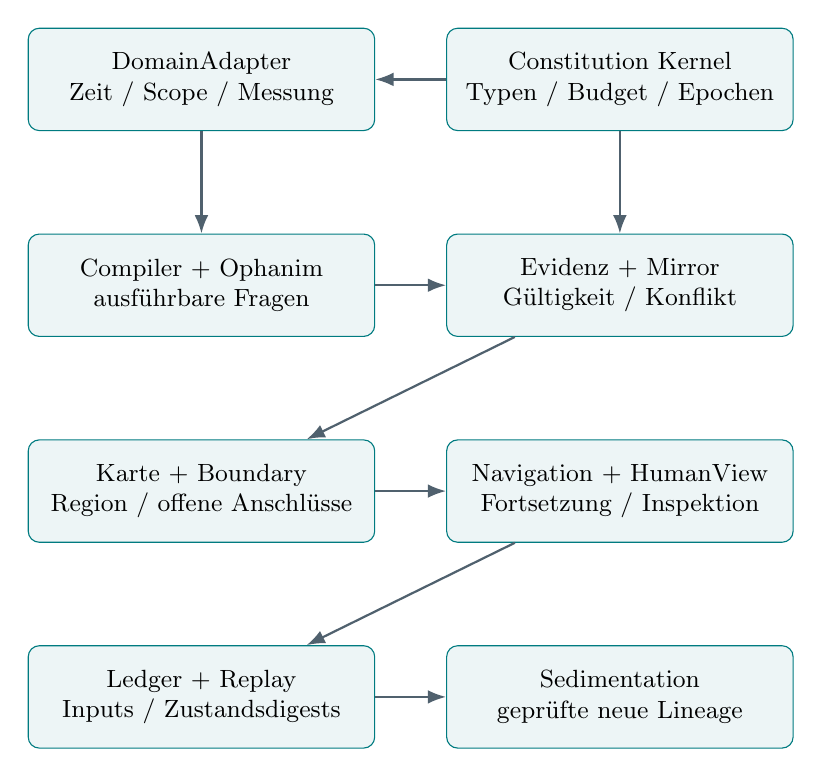
\begin{tikzpicture}[font=\small,box/.style={draw=accent,rounded corners,fill=pale,
minimum width=44mm,minimum height=13mm,align=center},
arr/.style={-{Latex},thick,color=muted}]
\node[box] (adapter) {DomainAdapter\\Zeit / Scope / Messung};
\node[box,right=9mm of adapter] (kernel) {Constitution Kernel\\Typen / Budget / Epochen};
\node[box,below=13mm of adapter] (sensor) {Compiler + Ophanim\\ausführbare Fragen};
\node[box,right=9mm of sensor] (evidence) {Evidenz + Mirror\\Gültigkeit / Konflikt};
\node[box,below=13mm of sensor] (map) {Karte + Boundary\\Region / offene Anschlüsse};
\node[box,right=9mm of map] (nav) {Navigation + HumanView\\Fortsetzung / Inspektion};
\node[box,below=13mm of map] (ledger) {Ledger + Replay\\Inputs / Zustandsdigests};
\node[box,right=9mm of ledger] (slow) {Sedimentation\\geprüfte neue Lineage};
\draw[arr] (kernel)--(adapter);
\draw[arr] (adapter)--(sensor);
\draw[arr] (kernel)--(evidence);
\draw[arr] (sensor)--(evidence);
\draw[arr] (evidence)--(map);
\draw[arr] (map)--(nav);
\draw[arr] (nav)--(ledger);
\draw[arr] (ledger)--(slow);
\end{tikzpicture}
\end{center}

Die Zeichnung beschreibt Rollen und Hauptabhängigkeiten. Im
ausführbaren Profil liegen Kernel, Evidenzverwaltung, Graphregion und
Navigation in einem deterministischen Prozess. Ihre Datenverträge
ermöglichen eine spätere Aufteilung auf Dienste oder Rust-Crates.

\subsection{Autorität über Aussagen}
Ein Adapter berichtet: Quelle $s$ meldete $y$ zur Zeit $t$ unter
Vertrag $a$. Der Compiler prüft die Bindung an das aktive Profil.
Die Evidenzverwaltung entscheidet über aktuelle Verwendbarkeit.
Die Modellschicht erzeugt abgeleitete Aussagen. Der Compositor darf
deren epistemische Klasse nicht erhöhen.

\subsection{Autorität über Wirkungen}
Für reale Eingriffe benötigt das Gesamtsystem einen separaten Effect Port:
\[
\mathrm{Measure}\to\mathrm{Evaluate}\to\mathrm{Propose}
\to\mathrm{Gate}\to\mathrm{Apply}\to\mathrm{Receipt}.
\]
Der Referenzkern erzeugt Modellnavigation und Sondenvorschläge.
Die neue Sessionruntime bindet daraus ausgewählte Messfragen an
konkrete lesende Dateisystemabfragen. ADVANCE bleibt eine
Modellausgabe. Ein allgemeiner schreibender Aktuator ist nicht enthalten.

\nextsection{03 / EPISTEMISCHE ABI}{Aussagetypen und orthogonale Attribute}
Ein Perzeptionsrecord einer Aussage $p$ lautet
\[
p=(q,z,v,f,a,\nu,\mathcal W,\mathcal D,\sigma),
\]
mit Frage $q$, epistemischer Klasse $z$, Wert $v$, Faktizität $f$,
Verfügbarkeit $a$, Gültigkeit $\nu$, Witnesses $\mathcal W$,
Abhängigkeitsinformation $\mathcal D$ und Scope $\sigma$.

\begin{tabularx}{\linewidth}{@{}lY@{}}
\toprule
Achse & Bedeutung und Werte\\\midrule
Epistemische Klasse & $\{\Known,\Ambiguous,\Unknown,\OOS,\Invalid\}$\\
Wert & Im Profil $\{\mathrm{true},\mathrm{false},\bot\}$;
$\bot$ bezeichnet einen nicht freigegebenen Modellwert.\\
Faktizität & Observed, Derived, Counterfactual; Rollen im
Erzeugungsweg. Der Kern projiziert Derived-Modellrecords.\\
Verfügbarkeit & observed, occluded, not\_observed; Quellen können
verschiedene Verfügbarkeiten tragen.\\
Gültigkeit & Zeitfenster, Modell-, Kalibrierungs-, Scope- und
Framebindung; im Profil Zeitfenster plus feste Runbindung.\\
Herkunft & Inhaltsadressierter Modellrecord mit Beobachtungsreferenzen.\\
\bottomrule
\end{tabularx}

\Known{} bedeutet, dass die vorgeschriebenen Kriterien für einen
eindeutigen aktuellen Modellwert erfüllt sind. \Ambiguous{} bezeichnet
aktive widersprüchliche zulässige Aussagen. \Unknown{} bezeichnet
unzureichende Bestimmtheit. \OOS{} bezeichnet eine Frage außerhalb
des Scopes. \Invalid{} bedeutet im Profil: Es gibt aktuell ungültig
markierte Beiträge, aber keine gültige beobachtete boolesche Aussage.

Ein bekannter falscher Wert bleibt \Known. Eine verdeckte Stelle kann
epistemisch unbekannt sein; eine andere gültige Quelle kann sie trotzdem
bestimmen. Deshalb gelten folgende Identifikationen ausdrücklich nicht:
\[
\Unknown=\mathrm{false},\qquad
\mathrm{not\_observed}=\mathrm{absent},\qquad
\mathrm{occluded}=\Unknown.
\]

\subsection{Support ohne erfundene Confidence}
Ein Quellenquorum oder Matchingwert ist keine kalibrierte
Wahrscheinlichkeit. Das Profil gibt keine Prozent-Confidence aus.
Der Support besteht aus benannten, deklarierten Abhängigkeitsgruppen.
Eine falsche Gruppendeklaration bleibt eine falsche Modellannahme.
Die Sichtbarkeit von Herkunft macht diese Annahme prüfbar.

\nextsection{04 / ZEITVERTRAG}{Aktive Evidenz und Mirror-Erneuerung}
Eine Beobachtung enthält
\[
e=(id,q,s,y,t_e,t_a,\mathrm{quality},\mathrm{visibility},\mathrm{label}),
\]
mit Ereigniszeit $t_e$ und Aufnahmetakt $t_a$. Es gilt $t_e\leq t_a$.
Aufnahmetakte müssen im Run monoton sein. Das Zeitmaß wird vom
Adapterprofil gebunden.

Für Quelle $s$ und Frage $q$ sei
\[
m_{s,q}=\max\{t_e:e\text{ wurde für }(s,q)\text{ angenommen}\}.
\]
Die aktuelle Kanalspitze enthält alle Records mit $t_e=m_{s,q}$.
Gleichzeitige widersprüchliche Werte werden nicht durch eine
ID-Sortierung aufgelöst. Für Time-to-live $\Delta>0$ und explizite
Rücknahmen $R_t$ ist
\[
\E_t(q)=\{e:t_e=m_{s,q},\ e.id\notin R_t,\ 0\leq t-t_e<\Delta\}.
\]
Nur gültige beobachtete Beiträge bilden $\E_t^{\rm claim}(q)$.
Die Rücknahme der neuesten Beobachtung reaktiviert keine ältere
Beobachtung automatisch.

\subsection{Statischer und dynamischer Mirror}
Im statischen v3-Vertrag gilt
$\M_{t+1}=\M_t\cap C(e_{t+1})$ innerhalb eines festen Modells.
Für eine veränderliche Welt wird die aktuelle Faser aus den
gegenwärtig geltenden Constraints bestimmt:
\[
\M_t^{(m)}=\{x\in X_m:\forall e\in\E_t,\ C_m(e,x)=1\}.
\]
Neue Evidenz kann sie verkleinern. Ablauf, Rücknahme, Scope- oder
Modellwechsel können sie vergrößern. Historische Mirrorzustände
bleiben als vergangene Zustände adressierbar.

\begin{proposition}
Unter festem Modellraum und reinem Hinzufügen von Constraints
ist die Mirrorfolge monoton fallend. Nach Entfernen einer Bedingung
besteht diese Monotoniegarantie nicht.
\end{proposition}
\begin{proof}
Eine zusätzliche Schnittbedingung kann keine Elemente hinzufügen.
Nach Entfernen einer Bedingung können zuvor ausgeschlossene
Elemente alle verbleibenden Bedingungen erfüllen.
\end{proof}

Ein leerer Mirror $\M_t=\varnothing$ bezeichnet einen
Constraintkonflikt im Modell. Er ist keine eindeutige Rekonstruktion.
Das Profil gibt \Ambiguous{} aus und behält die Gegenbelege.
Ein weiterentwickelter Solver kann getrennte Reparaturhypothesen
führen; ihre Auswahl benötigt einen eigenen Modellvertrag.

\nextsection{05 / REFERENZSEMANTIK}{Ausführbare boolesche Klassifikation}
Sei $Y_q$ die Wertmenge aus $\E_t^{\rm claim}(q)$ und $D_q$ die
Menge ihrer deklarierten Quellengruppen. Für Mindestquorum $k$
werden die folgenden Regeln in dieser Reihenfolge ausgewertet:
\[
z(q)=
\begin{cases}
\OOS{} & q\notin\mathrm{Scope},\\
\Ambiguous{} & |Y_q|>1,\\
\Known{} & |Y_q|=1\land |D_q|\geq k,\\
\Invalid{} & \E_t^{\rm claim}(q)=\varnothing
\land\exists e\in\E_t(q):e.\mathrm{quality}=\mathrm{invalid},\\
\Unknown{} & \text{sonst}.
\end{cases}
\]
Nur für $z(q)=\Known$ wird ein boolescher Modellwert freigegeben.
Die lokale Kandidatenmenge ist
\[
M(q)=
\begin{cases}
\varnothing & |Y_q|>1,\\
Y_q & |Y_q|=1,\\
\{\mathrm{false},\mathrm{true}\} & |Y_q|=0.
\end{cases}
\]
Eine einzelne Quelle kann damit eine Hypothese einschränken,
ohne die Bestimmtheitsregel für \Known{} zu erfüllen.

\begin{proposition}[Quoruminvariante]
Jeder ausgegebene \Known-Record besitzt mindestens $k$ deklarierte
Supportgruppen und genau einen aktiven beobachteten Wert.
\end{proposition}
\begin{proof}
Die einzige Codeverzweigung, die \Known{} setzt, prüft genau diese
Bedingungen. Die vorangehende Konfliktverzweigung schließt
$|Y_q|>1$ aus. Rendering übernimmt dieselbe Klasse.
\end{proof}

Die Aussage gilt über Records und Deklarationen. Sie beweist weder
Sensorunabhängigkeit noch Außenweltwahrheit. Zwei Sensoren können
denselben systematischen Fehler teilen. Dies muss extern evaluiert werden.

Mehrfache Beiträge derselben Gruppe erhöhen $|D_q|$ nicht.
Das ist eine konservative Zählregel. Der umfassendere v3-Dependencyquotient
mit tatsächlichem effektivem Rang bleibt eine weitere Inferenzrolle.

\texttt{fresh} bedeutet: Mindestens ein aktueller Beitrag liegt vor.
\texttt{stale} bedeutet: Historie liegt vor, aber kein Beitrag ist aktiv.
\texttt{inactive\_reasons} unterscheidet EXPIRED und RETRACTED.
\texttt{none} bezeichnet fehlende Historie.
\texttt{valid\_until} gibt konservativ das früheste Ablaufdatum
der aktuell stützenden Beobachtungen an.

\nextsection{06 / KOMPILATION}{Genome, Operatorbindung und Normalform}
Das ausführbare Genome bindet Profilversion, Faktenraum, Quellen,
Scope, Ziel, Graphkanten, Operatorgene und Budgets.
Der Compiler akzeptiert ausschließlich diese vertikale Pipeline:
\begin{align*}
\mathrm{Observation}&\xrightarrow{\texttt{observe\_bool@1}}\mathrm{BooleanEvidence},\\
\mathrm{BooleanEvidence}&\xrightarrow{\texttt{classify\_bool@1}}\mathrm{Percept},\\
\mathrm{Percept}&\xrightarrow{\texttt{project\_view@1}}\mathrm{ViewObject}.
\end{align*}
Die Reihenfolge folgt aus typgeprüften Abhängigkeiten.
Operatorimplementierungen sind fest gebunden. Das Compilemanifest
enthält GenomeDigest, RegistryDigest, topologische Ausführungsordnung,
Kanonisierungsprofil und abstrakte Pipelinekosten.

\subsection{Idempotenz benötigt stärkere Voraussetzungen}
Die Idempotenz der zusammengesetzten v3-Normalform folgt nicht
allein aus idempotenten Teiloperationen. Auf $\{0,1,2\}$ seien
\[
C=(0\mapsto0,1\mapsto1,2\mapsto1),\qquad
R=(0\mapsto2,1\mapsto1,2\mapsto2).
\]
Beide Funktionen sind idempotent. Für $N=R\circ C$ gilt aber
$N(0)=2$ und $N(N(0))=1$.

\contract{Eine Normalform braucht eine charakterisierte Fixpunktmenge.
Nachfolgende Stufen müssen die Invarianten vorangehender Stufen
erhalten; alternativ ist ein terminierendes, konfluent normalisierendes
Verfahren erforderlich.}

Im Profil ist diese Menge explizit: eindeutige IDs, gültige
Signaturen, sortierte Fakten, eindeutige sortierte Kanten,
sortierte Abhängigkeiten und dieselbe topologische Geneordnung.
Erneute Kompilation erzeugt daher dasselbe Genome und Manifest;
dies wird separat getestet.

\subsection{Ophan als typisierter Prozessvertrag}
In der Zielarchitektur bindet ein Ophan Frage, Operatorversion,
Phase, Apertur, Laufidentität, Ressourcen und Evidenzausgabe.
Das Profil implementiert Aufnahme, Klassifikation, Projektion
und Sondenauswahl. Eine Rotorfaser-Runtime mit zyklischer
Expositionsdynamik folgt daraus allein nicht. Die neue Organruntime
konkretisiert einen endlichen Teil dieses Vertrags in den Abschnitten
22--24: Ihre Exposition verändert eine gebundene Sektorabfrage.

\nextsection{07 / KARTOGRAPHIE}{Drei Graphen und eine begründete Region}
Der \emph{Herkunftsgraph} verbindet Beobachtungen, Transformationen
und Modellrecords. Der \emph{Operationsgraph} beschreibt Beziehungen
im Domänenmodell. Der \emph{Darstellungsgraph} enthält sichtbare
Objekte und Layoutbeziehungen. Gleiche Zeichen auf dem Bildschirm
begründen keine Identität in einem dieser Graphen.

Im Referenzprofil ist der Operationsgraph $G_\Gamma=(Q,E_\Gamma)$
vorgegeben. Seine Kanten sind Deklarationen; der Kern entdeckt keine
unbekannten realen Verbindungen. Er bestimmt, welcher Teil des
Graphen durch aktuelle positive Knotenwerte zusammenhängend ist.

Definiere
\[
Q_t^+=\{q\in Q:z_t(q)=\Known\land v_t(q)=\mathrm{true}\}.
\]
Die operative Region ist
\[
\Omega_t=
\begin{cases}
\operatorname{Component}_c(G_\Gamma[Q_t^+]) & c\in Q_t^+,\\
\varnothing & \text{sonst}.
\end{cases}
\]
Die Frontier enthält alle außerhalb liegenden Nachbarn von $\Omega_t$.
Ein bekannter negativer Knoten kann dort liegen und behält seine Klasse.

\begin{proposition}
Jeder Knoten der Region ist aktuell positiv bestimmt und über
einen Pfad aktuell positiv bestimmter Knoten mit dem Zentrum verbunden.
\end{proposition}
\begin{proof}
Die Breitensuche beginnt nur in $Q_t^+$ und fügt ausschließlich
Nachbarn aus $Q_t^+$ hinzu. Ihr Suchbaum liefert für jeden
aufgenommenen Knoten einen entsprechenden Pfad.
\end{proof}

\subsection{Gluing benötigt zusätzliche Witnesses}
Rekonstruierte Patches benötigen tatsächliche Überlappungen,
Objektkorrespondenzen, Übergangsfunktionen, Zeit- und
Scopekompatibilität sowie Toleranzen. Paarweise Kompatibilität
genügt allgemein nicht zur globalen Verklebung. Auf Dreifachüberlappungen
ist beispielsweise
\[
T_{ik}\simeq T_{jk}\circ T_{ij}
\]
zu prüfen. Höhere Simplizes benötigen einen gemeinsamen Witness.
Die Referenzregion beansprucht keine solche Patch-, Nerven-
oder Sheaf-Konformität.

\nextsection{08 / STRUKTURVERTRÄGE}{Spektrum, Skala und Reflexion}
\subsection{Spektrale Mehrdeutigkeit}
Für eine reelle symmetrische Adjazenzmatrix $A$ gilt
\[
\operatorname{tr}(A^k)=\sum_i\lambda_i^k.
\]
Spurpotenzen derselben Matrix unterscheiden somit keine bezüglich
dieser Matrix kospektralen Graphen. Das v3-Referenzszenario E benötigt
einen zusätzlichen, spektral nicht bereits festgelegten Deskriptor.
Der Literaturanschluss ist van Dam und Haemers \cite{spectra}.

Ein konkretes Paar ist $K_{1,4}$ gegenüber $C_4\sqcup K_1$.
Beide besitzen das Spektrum $\{-2,0,0,0,2\}$.
Die Gradmultimengen $\{4,1,1,1,1\}$ und $\{2,2,2,2,0\}$
trennen dieses Paar. Daraus folgt keine allgemeine Vollständigkeit
des Gradwitnesses.

\subsection{Verlustbehaftete Skalenabbildung}
Ist $Q:X_{\rm fine}\to X_{\rm coarse}$ nicht injektiv, kann
ein deterministischer Lift $L$ nicht für alle $x$ die Identität
$L(Q(x))=x$ erfüllen. Ein gültiger Roundtrip lautet stattdessen
\[
Q(L(y))=y
\quad\text{oder}\quad
L(Q(x))\sim_Q x,\qquad x\sim_Q x'\iff Q(x)=Q(x').
\]
Für exakte feinere Identität sind Residualdaten $r$ mit
$L(Q(x),r)=x$ erforderlich. Ein UI-Zoom ist kein ScaleWitness.

\subsection{Reflexionsalgebra und Evidenzbegründung}
Eine selbstadjungierte Involution $R=R^\ast$, $R^2=I$ erzeugt
orthogonale Projektoren $P_\pm=(I\pm R)/2$. Die Gleichungen allein
bestimmen keine evidenzmäßig zulässige Weltregion.

Für einen bereits begründeten diskreten Bereich $\Omega\subseteq Q$
kann man auf $\R^Q$ setzen:
\[
P_\Omega=\operatorname{diag}(1_{q\in\Omega}),\qquad
R_\Omega=2P_\Omega-I.
\]
Dann ist $R_\Omega$ selbstadjungiert und involutiv. Der
Algebra-Witness kodiert die Bereichswahl; die Evidenzbegründung
stammt aus dem separaten Regionvertrag. Der Referenzkern
implementiert die Region, aber keine räumliche Reflexionsgeometrie.

\nextsection{09 / ATTRAKTORNAVIGATION}{Fortsetzung und budgetierte Messfragen}
Ein Zielwechsel erhöht die Zielepoche und verändert Prioritäten.
Evidenzrecords werden dadurch nicht umgeschrieben. Im Profil ist der
Attraktor ein benannter Zielknoten. ADVANCE erfordert einen aktuell
positiv bestimmten Pfad vom Zentrum zum Ziel und verfügbare Framebindung.

Der Pfad beschreibt eine Fortsetzung im vorgegebenen Operationsgraphen.
Bei Systemkomponenten ist dies eine Inspektions- oder
Abhängigkeitsrichtung. Er ist keine automatisch zulässige
Netzwerkroute oder physische Bewegungsbahn.

\subsection{Transparente Sondenheuristik}
Für jede noch nicht bekannte Frage im Scope wird ein Kandidat pro
bevorzugter Quelle erzeugt. Quellen aus noch nicht vertretenen
deklarierten Gruppen werden bevorzugt. Wenn solche Gruppen fehlen,
wird eine erneute Beobachtung aus vorhandenen Quellen vorgeschlagen.

Die ganzzahlige Priorität ist
\begin{align*}
S(q)={}&20+40\,1_{\rm Konflikt}+30\,1_{\rm Frontier}\\
&+\max(0,25-5d_\Gamma(q,a))+10\,1_{\rm stale}.
\end{align*}
$a$ ist das Ziel; $d_\Gamma$ ist die Distanz im deklarierten Graphen.
Fehlende Erreichbarkeit erhält keine Zielnähe.
Die sortierte Kandidatenfolge nutzt Fakten-ID und Quellen-ID als
Tie-Breaker. Pro Frage wird höchstens ein Vorschlag aufgenommen;
die Pipelinekosten bleiben im Probenbudget.

\contract{Der Score ist eine offengelegte Heuristik. Er darf nicht
als gemessener Informationsgewinn, Erfolgswahrscheinlichkeit oder
Nachweis globaler Optimalität ausgegeben werden.}

Die Kosten sind abstrakte Einheiten. Die Sessionruntime ergänzt diese
Kernheuristik um Fälligkeit und faire Bedienung: Unter zulässigen
Endpunkten wird der am längsten nicht versuchte zuerst gewählt.
Die Kernpriorität dient als nachgeordneter Tie-Breaker.
Auch bestimmte Aussagen erhalten geplante Erneuerungsmessungen.
Ein dispatch erzeugt eine reale, zeitlich begrenzte Dateisystemabfrage.

\subsection{Allgemeiner Tangentenkompass}
Ein kontinuierliches Profil darf
$v^\parallel=-\Pi_{\rm adm}\nabla V$ verwenden, wenn Chart,
Differentialstruktur, Metrik, Potential und Projektion spezifiziert sind.
Auf Graphen reicht eine diskrete Aktionsbewertung. Eine endliche
Skalenleiter besitzt keine gewöhnlichen Tangentialräume;
ihre vertikale Komponente ist eine Auswahl typisierter Übergänge.

\nextsection{10 / HUMANVIEW}{Darstellung ohne epistemische Aufwertung}
Ein sichtbares Objekt enthält
\[
(id,\mathrm{machineRef},z,v,f,\mathrm{sourceRefs},
\mathrm{freshness},\mathrm{visibility},\mathrm{frame},h,\mathrm{interaction}).
\]
Die HTML-Ansicht projiziert diese Records. Sie erzeugt keine eigene
Klassifikation aus einer anderen Evidenzheuristik.

\begin{tabularx}{\linewidth}{@{}lY@{}}
\toprule
Darstellung & Normative Bedeutung\\\midrule
Türkis: Known / true & Aktuell positiv freigegebener Modellwert.\\
Rot: Known / false & Aktuell negativ freigegebener Modellwert.\\
Amber: Ambiguous & Aktiver Widerspruch gültiger Aussagen.\\
Grau: Unknown & Unzureichende Bestimmtheit; Ursache ist inspizierbar.\\
OutOfScope / Invalid & Explizite Texte ergänzen die Farbgebung.\\
Helle Kanten & Verbindung zweier Knoten in der aktuellen Region.\\
Gestrichelte Zielkontur & Gebundenes Ziel, unabhängig von seiner Wahrheit.\\
Zeitschieber & Auswahl eines gespeicherten früheren Kernzustands.\\
Sondenvorschlag & Frage, Quelle, Scorekomponenten und Kosten.\\
\bottomrule
\end{tabularx}

\subsection{Projektionsinvariante}
Für jede dargestellte Frage gilt
\[
z_V(q)=z_M(q),\qquad v_V(q)=v_M(q),\qquad
\mathrm{refs}_V(q)=\mathrm{refs}_M(q).
\]
Ein künftiger LOD-Compositor darf ausblenden und aggregieren.
Er muss offene Anteile und Konflikte erhalten. Zehn bekannte und
eine unbekannte Komponente ergeben nicht allein aufgrund der
Mehrheit eine bekannte Sammelaussage.

\subsection{Zeit- und Framebezug}
Das Layout verwendet \texttt{machine\_graph} und
\texttt{world\_registered=false}. Bildschirmpositionen sind
Darstellungskoordinaten. Ein simuliertes Trackingflag unterdrückt
bei Verlust die Navigation, implementiert aber keinen Tracker.

Frische im Replay bezieht sich auf die Zeit des ausgewählten
Snapshots. Eine alte Datei wird damit nicht zu einer Livebeobachtung.
Die Oberfläche kennzeichnet den aufgezeichneten Lauf.
Der ursprüngliche Compositor markiert importierte Runs als
ungeprüfte Ansicht. Der neue Sessionexport prüft das Journal
durch erneute Ausführung, bevor er die Offlineansicht erzeugt.
Der Live- und Deltavertrag steht in Abschnitt 18.

\nextsection{11 / BETRIEBSVERTRAG}{Transaktionen, Ressourcen und Epochen}
Ein wohlgeformtes Ereignis wird auf einer Zustandskopie verarbeitet.
Nach erfolgreicher Prüfung wird sie übernommen. Bei einem
inhaltlichen Fehler bleibt der Zustand unverändert; ein REJECTED-Trace
benennt den Fehler:
\[
\operatorname{Step}(S,e)=
\begin{cases}
(F(S,e),\mathrm{COMMITTED}) & \mathrm{Valid}(S,e),\\
(S,\mathrm{REJECTED},r) & \text{sonst}.
\end{cases}
\]
Transportfehler vor dem akzeptierten Ereignisraum -- unzulässige
JSON-Typen, überschrittene Bytebudgets oder ID-Kollisionen --
beenden den CLI-Aufruf. Sie erzeugen keinen fiktiv erfolgreichen Puls.
Ein identisches erneut gesendetes Ereignis ist idempotent und
erzeugt keinen zusätzlichen Trace.

\subsection{Ressourcen}
Das Profil erlaubt höchstens 128 Fragen, 64 Quellen, 64 Gene und
512 deklarierte Kanten. Das Beispielgenome begrenzt den Run
auf 512 Ereignisse, 4096 kanonische Bytes pro Ereignis und
sechs abstrakte Sondenkosteneinheiten pro Zustand.
Das neue Dateisessionprofil bindet eine eigene Ereigniskapazität
und zusätzliche Queue- und Laufgrenzen gemäß Abschnitt 16.

Der Referenzalgorithmus scannt die begrenzte Historie und schreibt
vollständige Snapshots. Bei $F$ Fragen, $S$ Quellen und $H$
historischen Records kostet die direkte Klassifikation in dieser
Implementierung im ungünstigen Fall $O(FSH)$; Graphsuche kostet
$O(F+|E_\Gamma|)$. Die gespeicherten Trace- und Referenzlisten
wachsen über einen Run. Ein Produktionskern benötigt Indizes,
inkrementelle Materialisierung und kompakte Checkpoints.
Harte Echtzeit wird nicht beansprucht.

\subsection{Statusräume}
COMMITTED und REJECTED bezeichnen Eingabetransaktionen.
ADVANCE, PROBE, HOLD und REANCHOR bezeichnen die Navigation.
Ein gültiger Tick kann COMMITTED sein und danach HOLD ergeben.
Die weiteren v3-Status REACQUIRE, RESIDUAL, ACT, STOP und FAIL
sind nicht vollständig in diesem Profil implementiert.

\subsection{Epochen}
Genome und Registry bleiben im Run unverändert. Zielevents erhöhen
die Zielepoche. Wechsel des Trackingflags erhöhen die Frameepoche.
Kalibrierungs-, Modell- und Scopeänderungen benötigen in der
erweiterten Runtime eigene Epochen sowie Revalidierung abhängiger Records.

\nextsection{12 / REPLAY}{Kanonisierung, Integrität und deterministisches Gedächtnis}
L2-CANON-1 erlaubt ASCII-Strings, ASCII-Schlüssel, Boolean, Null,
Arrays, Objekte und ganze Zahlen im Bereich
$[-(2^{53}-1),2^{53}-1]$. Fließkommazahlen werden abgewiesen.
Objektschlüssel sind sortiert, zusätzliche Leerzeichen entfernt.
Doppelte JSON-Schlüssel werden beim Parsen abgewiesen.

RFC 8785 spezifiziert ein umfassenderes JSON-Kanonisierungsverfahren
einschließlich Zahlen- und Unicoderegeln \cite{jcs}. Das eingeschränkte
Profil besitzt einen eigenen Namen und beansprucht keine allgemeine
RFC-8785-Konformität.

\subsection{Digests ohne Selbstreferenz}
Für Payload $x$ und Recordtyp $\tau$ gilt
\[
h_\tau(x)=\mathrm{SHA256}
\big(\operatorname{Canon}([\mathrm{Profile},\tau,x])\big).
\]
Der Digest wird vor dem Hinzufügen seines eigenen Feldes gebildet.
Ein StateDigest enthält keinen Ledgerkopf, der wiederum von
diesem StateDigest abhängt. Ein Trace bindet
\[
(\mathrm{index},\mathrm{input},\mathrm{pre},\mathrm{post},
\mathrm{outcome},\mathrm{residuals},\mathrm{parent}).
\]

Replay kompiliert das Genome neu, führt die vollständige Eingabefolge
erneut aus und vergleicht Manifest, Anfangszustand, Tracefolge und
sämtliche Snapshots. Ein neu berechneter äußerer Hash über
manipulierte Renderrecords genügt deshalb nicht für ein erfolgreiches Replay.

\begin{proposition}
Bei gleicher Kernelversion und gleicher akzeptierter Eingabefolge
erzeugt der Kern dieselbe bytekanonische Bundleklasse.
\end{proposition}
\begin{proof}
Kanonisierung, Compileordnung, Klassifikation, Graphsuche und
Tie-Breaker sind deterministisch. Der Kern nutzt weder externe Uhren
noch Zufall. Induktion über die Eingabefolge liefert identische
Zustände und Traces. Ein Adapter schreibt gemessene Zeit zuvor als
gewöhnliche Eingabe in den Run.
\end{proof}

Hashverkettung und Replay prüfen interne Integrität relativ zu einem
bekannten Artefakt. Sie authentifizieren keine Sensoren. Eine vollständig
neu erzeugte konsistente Geschichte benötigt externe Signaturen,
Zeitanker oder unabhängige Zeugen, um ihre Herkunft zu belegen.

\nextsection{13 / PHYSISCHER TRÄGER}{Rotorfaser, Gyrosphäre und XR-Anschluss}
Die v3-Rotorfaser strukturiert eine zyklische Wahrnehmungsfrage über
Orientierungen. Ein räumliches Ausführungsprofil muss mindestens
Basisraum, Faser, Expositionsfunktion, Sensorantwort, Diskretisierung
und Messkosten festlegen:
\[
O_i=(\mathcal A_i,S^1,\theta_i,\mathrm{Expose}_i,
\mathrm{Measure}_i,\mathrm{Witness}_i,\beta_i).
\]
Eine Änderung von $\theta_i$ muss eine definierte Änderung der
Messfrage oder des Trägers besitzen. Kreisende Darstellungsobjekte
allein erfüllen diesen Vertrag nicht.

\subsection{720-Grad-Semantik}
Für den Quaternionenlift gilt
$\pi(q)=\pi(-q)$ unter $\pi:SU(2)\to SO(3)$.
Ein pfadgebundener Lift kann zusätzliche Verlaufsinformation tragen.
Ein isoliertes Orientierungsbild bestimmt diese Verlaufsklasse
nicht ohne weitere Festlegung. Der boolesche Referenzkern
führt keine Quaternionen und keine 720-Grad-Witnesses.

\subsection{Registrierter Framegraph}
Eine Transformationskante benötigt
\[
(F_i,F_j,T_{ij},t,\mathrm{CalibrationRef},U_{ij},\mathrm{Validity}).
\]
Pflichtfelder sind Einheiten, Koordinatenkonventionen,
Unsicherheitsdarstellung, Uhrenzuordnung und Ausfallbehandlung.
Ein linearisiertes Profil unabhängiger lokaler Fehler kann
$\Sigma_y=J\Sigma_xJ^\top+\Sigma_T$ verwenden.
Abhängige Fehler benötigen entsprechende Kreuzterme.

\subsection{Verlust und Wiedererfassung}
Abgelaufene Posen dürfen keine scheinbar stabile Weltregistrierung
tragen. Bei Überschreitung des Framefehlers wird weltregistrierte
Navigation zurückgenommen. Modellinspektion und historische
Ansicht können verfügbar bleiben. Wiedererfassung erzeugt
eine neue Framebindung und revalidiert abhängige Objekte.

Der Referenztest schaltet ein Trackingflag aus und wieder ein.
Er prüft die Kernreaktion, nicht Genauigkeit oder Latenz eines
realen Headsets. FrameRegistrationError, DisplayLatency,
Occlusion und InteractionRoundtrip benötigen einen eigenen
Carrier-Benchmark.

\nextsection{14 / WIRKUNG UND EVOLUTION}{Effect Port und Sedimentation}
Ein produktiver Effect Port benötigt einen konkreten Plan
\[
P=(id,\mathrm{stateRef},\mathrm{epoch},\mathrm{action},
\mathrm{preconditions},\mathrm{capability},\mathrm{expiry},\mathrm{nonce}).
\]
Eine Freigabe ist an diesen Plan gebunden. Vor Ausführung werden
Zustand, Zielepoche, Gültigkeit und Capability erneut geprüft.
Wiederholte Aufträge benötigen einen Idempotenzschlüssel.

Receipts unterscheiden \emph{versucht}, \emph{vom Träger bestätigt},
\emph{unabhängig nachbeobachtet}, \emph{fehlgeschlagen} und
\emph{unbekannter Ausgang}. Fehlende Bestätigung beweist keine
ausgebliebene Wirkung. Reconciliation erzeugt gegebenenfalls
eine neue Beobachtungsaufgabe.

Das Paket enthält keinen allgemeinen schreibenden Effect Port und
keine implementierte Capability-Prüfung. Die Sessionruntime führt
gebundene lesende Messungen aus. Ihr Prozess-Timeout und ihre
Eingabeprüfung ersetzen keine Betriebssystem-Sandbox.

\subsection{Getrennte strukturelle Evolution}
Sedimentation verarbeitet versiegelte Runs und erzeugt
\[
SC=(\mathrm{parents},\mathrm{delta},\mathrm{trainingRefs},
\mathrm{heldoutRefs},\mathrm{metrics},\mathrm{ablation},
\mathrm{migration},\mathrm{residues}).
\]
Ein Kandidat wird gegenüber derselben Aufgabe und festgehaltenen
Baselines geprüft. Trainings- und unabhängige Prüfdaten dürfen
nicht stillschweigend dieselbe Rolle übernehmen.

Eine mögliche lexikographische Evaluationsordnung ist
\[
\min\big(\mathrm{ContractViolations},\mathrm{FalseCertainty},
\mathrm{MissedCriticalUnknown},\mathrm{Cost}\big).
\]
Gewichte und Freigabeschwellen müssen vor dem Vergleich feststehen.
Weniger offene Aussagen sind nur dann ein Fortschritt, wenn
dadurch keine unbegründete Sicherheit entsteht.

Diese Fassung enthält den Vertrag und Reanalyse durch neue Runs.
Automatische Mutation, Shadow-Deployment, Migration und
gemessener Transfer bleiben Implementierungsaufgaben.


\nextsection{15 / GESCHLOSSENER ZYKLUS}{Von der Messfrage zur erneuerten Wahrnehmung}
Die Abschnitte 15--19 konkretisieren den gemeinsamen Systemvertrag
im kompatiblen Dateisessionprofil 0.2.0. Das Organprofil erweitert
ihn ab Abschnitt 22 um Instrumentenidentität und Exposition.
Die Dateiruntime führt die folgende Rückkopplung tatsächlich aus:
\[
\mathrm{Need}\to\mathrm{Request}\to\mathrm{AdapterReceipt}
\to\mathrm{Evidence}\to\mathrm{Percept}\to\mathrm{ViewDelta}.
\]
Der nächste Need wird aus dem aktualisierten Zustand und den
Fälligkeiten der Endpunkte berechnet. Die Umweltereignisse im
Integrationslauf werden ausschließlich vom Testharness verursacht;
die Runtime erhält keine Erfolgsetiketten und verändert die
beobachteten Dateien nicht.

\subsection{Gebundener Messvertrag}
Jeder Endpunkt bindet Fact, Quelle, Pfad und eine feste Frage:
\texttt{is\_file} oder \texttt{is\_dir}. Ein Request enthält ID,
Endpunkt, Messfrage, Ausstellungszeit, Deadline, StateRef,
Ziel- und Frameepoche, Grund, Kosten und
\texttt{effect=READ\_METADATA}. Es gibt höchstens einen
offenen Request. Die aktuelle Implementierung startet hierfür
einen eigenen Python-Prozess ohne Shell.

\begin{tabularx}{\linewidth}{@{}lY@{}}
\toprule
Receipt & Operative Bedeutung\\\midrule
OK, true/false & gültige gemessene Aussage; false bedeutet
beobachtetes Nichtvorliegen, nicht fehlende Evidenz.\\
TIMEOUT & fehlendes verwertbares Resultat; im Einquellenprofil
wird die betroffene Aussage Unknown.\\
ERROR & fehlerhafter Messzugriff oder Protokollfehler;
im Einquellenprofil wird die Aussage Invalid.\\
SUPERSEDED & die Antwort bleibt im Journal, erhält aber keine
neue operative Evidenzbindung unter einer geänderten Epoche.\\
\bottomrule
\end{tabularx}

Eine Antwort muss zum offenen Request gehören. Doppelte oder
fremde Receipts werden abgewiesen. Messzeit und Eingang müssen
innerhalb des gebundenen Zeitvertrags liegen. Ein nach Deadline
eingetroffenes OK wird als Timeout behandelt. Bei Ziel- oder
Framewechsel, Pause oder verlorenem Tracking kann die frühere
Requestbindung keine neue Evidenz mehr begründen.

\subsection{Erneuerung und faire Bedienung}
Bestimmte Aussagen werden nach \texttt{refresh\_ms} erneut
gemessen. Fehlerhafte oder fehlende Antworten erhalten
\texttt{retry\_ms}. Unter fälligen Endpunkten gewinnt zunächst
der älteste Versuch, dann die Kernpriorität, dann die stabile ID.
Das verhindert dauerhafte Verdrängung fälliger Endpunkte im
endlichen Ein-Worker-Profil. Es beweist keinen optimalen
Informationsgewinn und keine garantierte Erneuerung vor TTL,
wenn die Messkapazität dafür nicht ausreicht.

\nextsection{16 / BETRIEBSVERTRAG}{Ereignisdienst, Invalidierung und Grenzen}
\subsection{Ein Eigentümer des Zustands}
Ein Worker besitzt die Sessionmaschine. HTTP-Anfragen liefern
Steueraufträge in eine begrenzte Queue. Ein Auftrag wird als
\texttt{QUEUED} bestätigt; erst sein späterer Commit verändert
den Zustand. Bei voller Queue antwortet der Dienst mit HTTP 429.
Pause, Zielwechsel, Tracking und Stop sind die vorhandenen
Steuerbefehle. Es gibt keinen HTTP-Eingang für beliebige
Beobachtungen oder ausführbare Programme.

Die Pause verhindert weitere Messaufträge; Ticks laufen weiter
und lassen Evidenz verfallen. Bereits laufende Messungen
begrenzen die Reaktionszeit der Steuerung: Der Worker verarbeitet
den nächsten Steuerauftrag nach Abschluss oder Timeout.
Ticks werden während dieses synchronen Wartens ebenfalls erst
danach verarbeitet. Das Profil beansprucht keine harte Echtzeit.

\subsection{Selektive Revalidierung}
Der innere Kern speichert Perzepte einschließlich ihres nächsten
Verfallszeitpunkts. Beobachtung und Rücknahme invalidieren den
betroffenen Fact; Zeitschritte invalidieren Perzepte mit
überschrittener Gültigkeit. Die Zustände werden gegen den
ursprünglichen vollständigen Interpreter verglichen.

Diese Optimierung betrifft lokale Perzeptklassifikation.
Ein neu berechneter Fact kann seine bisherige Historie durchsuchen.
Globale Graphregion, Navigation und Snapshots werden weiterhin
neu aufgebaut; Transaktionen kopieren Zustand. Es handelt sich
deshalb nicht um einen vollständig inkrementellen Graphsolver
oder um unbegrenzt skalierende Streaming-Speicherung.

\subsection{Gebundene Ressourcen}
Der Dateiconfigurator erzeugt standardmäßig TTL 2000\,ms,
Erneuerung 500\,ms, Timeout 500\,ms und Ticks von 50\,ms.
Die Steuerqueue umfasst 16 Aufträge, der Delta-Ring 64 Übergänge.
Ein Lauf ist standardmäßig auf 600 Sessionübergänge begrenzt.
Der innere Kernel erhält dazu eine entsprechend größere
Ereigniskapazität; sie ist nicht mit der Zahl der Sessionübergänge
identisch. Der Worker reserviert Platz für den geordneten Stop.

Die Laufzeitoption von 60 Sekunden ist eine zusätzliche Obergrenze;
das Übergangsbudget kann den Lauf früher beenden. Resume erhält
das gebundene Budget und verbrauchte Zähler. Für einen neuen
Budgetabschnitt wird ein neues Journal angelegt. Eine automatische
Rotation mit durchgehender Lineage gehört zum Organprofil
gemäß Abschnitt 25; das Dateiprofil behält seine einzelne Journaldatei.

Pfade und IDs unterliegen dem ASCII-Kanonisierungsprofil.
Der Dateiconfigurator akzeptiert bis zu 32 Dateien, der allgemeine
Sessionvertrag bis zu 64 gebundene Endpunkte. Dateiinhalte,
rekursive Verzeichnisüberwachung und selbstständiges Entdecken
neuer Knoten sind nicht Bestandteil dieses Adapters.

\nextsection{17 / FORTSETZBARES GEDÄCHTNIS}{Journal, Checkpoint und Wiederanlauf}
Die Session besitzt eine eigene reine Übergangsfunktion.
Ein akzeptierter Übergang wird auf einer Kandidatenkopie
berechnet und als JSONL-Record geschrieben. Erst nach
Flush und \texttt{fsync} wird der neue Zustand veröffentlicht:
\[
\mathrm{ComputeCandidate}\to\mathrm{Append}\to\mathrm{fsync}
\to\mathrm{Publish}.
\]
Ein Schreibfehler stoppt den Dienst mit Fehlerstatus; ein nicht
dauerhaft bestätigter Kandidat wird nicht als aktueller Zustand
publiziert. Dies ist ein Dateisystemvertrag, keine universelle
Garantie gegen jeden Hardware- oder Stromausfall.

\subsection{Replay als erneute Ausführung}
Der Header bindet normalisierte Konfiguration und Anfangszustand.
Jeder Übergang bindet Folgeindex, Eingabe, PreState, PostState,
Ausgabe, Vorgängerdigest und eigenen Digest. Replay führt
alle vollständigen Records erneut aus und vergleicht ihre
Semantik. Auch ein nachträglich neu gehashtes, semantisch
manipuliertes Journal wird durch den Vergleich erkannt.

Ein atomar ersetzter Checkpoint enthält Zustand, Journalposition
und Kopf. In dieser Fassung wird er durch vollständiges Replay
geprüft. Er ist ein Wiederherstellungsnachweis; ein vertrauenswürdiger
Schnellstart ohne Replay des Präfixes ist noch nicht implementiert.

\subsection{Abgerissene Schreibvorgänge}
Ein vollständiger, korrupter JSONL-Record wird abgewiesen.
Ein unvollständiges letztes Fragment wird beim normalen Replay
ebenfalls abgewiesen. Der explizite Wiederanlauf prüft das
vollständige Präfix, sichert das Fragment unverändert in einer
\texttt{.torn}-Datei und setzt erst dann das Journal auf das
geprüfte Präfix zurück. Eine vorhandene Fragmentdatei wird
nicht stillschweigend überschrieben.

\subsection{Neue Bindung nach einem Prozessende}
Die Host-Uhr wird beim Replay nicht gelesen. Beim realen Resume
wird die neue Sessionzeit konservativ auf den letzten Takt plus
TTL plus eine Millisekunde gesetzt. Der Resume-Übergang lässt
somit alle bisherigen Beobachtungen verfallen, verwirft die
operative Bindung eines gegebenenfalls offenen Requests und
plant frische Messungen. Er behauptet keine Kenntnis der
tatsächlich vergangenen Offlinezeit.

Konfiguration und Journalidentität bleiben gebunden.
Hashverkettung bestätigt weiterhin nur interne Konsistenz,
nicht die Authentizität der ursprünglichen Umweltmessungen.

\nextsection{18 / LIVE SECOND LAYER}{Projektion, Deltavertrag und Offlineansicht}
Der Live-Compositor bezieht ausschließlich Maschinenprojektionen
vom lokalen Dienst. Sichtbar sind epistemische Klasse, Wert,
Quellenbeleg, Gültigkeit, operative Region, nächste Messfrage,
offener Request und letzter Ausgang. Die eingebettete Offlineansicht
enthält dieselbe Projektion aus einem vollständig geprüften Journal.

\subsection{Deltaverkettung}
Ein ViewDelta bindet Sequenz und Zustandsdigest vor und nach
dem Übergang, geänderte und entfernte Objekte sowie aktuelle
Metadaten. Nur ein Delta mit passender Vorgängersequenz und
passendem Digest darf auf die vorhandene Ansicht angewendet werden.
Bei Lücke oder überlaufenem Ring liefert der Server einen
vollständigen Snapshot. Die Metadaten enthalten die aktuelle
Ziel- und Framebindung.

Die laufende Ansicht fragt den Dienst ungefähr alle 300\,ms ab.
Diese Abfrageperiode ist keine gemessene Gesamtlatenzgarantie.
Bei Verbindungsverlust wird der angehaltene Anzeigestand
als solcher gekennzeichnet. Ein STOPPED-Snapshot ist die
historische Endansicht des Laufs; ohne Runtime-Ticks wird er
nicht als neu gemessener gegenwärtiger Umweltzustand ausgegeben.

\subsection{Lokale Bindung}
Der HTTP-Dienst bindet ausschließlich an 127.0.0.1.
Host- und Origin-Prüfungen begrenzen fremde Browseraufrufe;
JSON-Steuerkörper sind auf 4096 Bytes begrenzt.
Diese Maßnahmen sind kein Mehrbenutzer-Authentisierungssystem.
Der Dienst ist für eine lokale Sitzung unter Kontrolle
des ausführenden Benutzers vorgesehen.

\subsection{Grenze des Darstellungsnachweises}
Der Integrationslauf prüft 43 tatsächlich über HTTP gelieferte
Projektionen gegen die Sessionmaschine. JavaScript-Prüfungen
führen die Ansichtslogik mit einer minimalen DOM-Testumgebung aus.
Eine visuelle Prüfung in einem echten Browser war in der
Erstellungsumgebung nicht verfügbar. Pixelgeometrie,
Browserkompatibilität und reale Eingabelatenz sind dadurch
nicht abschließend geprüft.

\nextsection{19 / REALER INTEGRATIONSLAUF}{Änderung, Verfall, Timeout und Wiedererfassung}
Der mitgelieferte Lauf verwendet zwei vom Harness erzeugte
Testdateien und ihren gemeinsamen Verzeichnisanker.
Die Runtime fragt ausschließlich Metadaten ab.
Das Quellenquorum beträgt eins; die Graphkanten sind
deklarierte Gruppierung, keine rekonstruierte Umwelttopologie.

\begin{tabularx}{\linewidth}{@{}rrY@{}}
\toprule
Sequenz & Takt/ms & Beobachtetes Ergebnis\\\midrule
9 & 126 & Beide Dateien und Verzeichnisanker Known true.\\
13 & 204 & Entfernte Datei Known false; Region kontrahiert.\\
23 & 392 & Wiederhergestellte Datei erneut Known true.\\
43 & 891 & Pause: alle drei Evidenzen abgelaufen, Region leer.\\
53 & 1087 & Automatische Wiedererfassung nach Aufhebung der Pause.\\
56 & 1369 & Real blockierter Messprozess beendet; Anker Unknown.\\
65 & 1571 & Erneute erfolgreiche Messung; Region wieder vollständig.\\
66 & 1603 & Geordneter STOPPED-Zustand und geprüfter Checkpoint.\\
\bottomrule
\end{tabularx}

Der Lauf enthält 14 Messaufträge, 66 akzeptierte Sessionübergänge,
43 geprüfte HTTP-Projektionen und 20 lokale Perzeptneuberechnungen.
Die Zeitspalte gibt Takte dieser konkreten Ausführung wieder.
Die Mutationszeitpunkte wurden nicht separat protokolliert;
aus der Tabelle wird deshalb keine Detektionslatenz abgeleitet.

Das Harness injiziert den blockierten Prozess ausdrücklich als
Fehlerfall. Der normale Messadapter verwendet ausschließlich den
festen Dateiabfrage-Worker. Weder HTTP noch Sessionkonfiguration
erlauben die Auswahl eines beliebigen Programms.

\subsection{Reproduktionsidentität}
Replay des gespeicherten Journals ergibt denselben Zustand:
\begin{lstlisting}
84f8fa361812bb653fd3b59a62fa58ac43716c0d4cbb2e242f24c699cecd5e95
\end{lstlisting}
Eine neue reale Ausführung hat andere Messzeiten und damit
andere Digests. Reproduzierbarkeit bedeutet hier identische
Übergangssemantik für dieselben aufgezeichneten Eingaben.
Eine erneute Abfrage der inzwischen veränderten Umwelt
ist ein neuer Versuch.

\nextsection{20 / VERIFIKATION}{Vertragstests und empirische Reichweite}
Die Ausgabe enthält 34 Kerntests, 27 Dateisessiontests und 36
Organprüfungen, insgesamt 97 Python-Tests. Sie prüfen Quellenquorum,
Rücknahme, alle epistemischen Klassen, Verfall, Region,
Transaktionsgrenzen und Replay. Ein reproduzierbarer
Kernlauf umfasst 120 generierte Ereignisse.

Die neuen Prüfungen umfassen gebundene und doppelte Receipts,
Epochenwechsel, faire Erneuerung, selektive Invalidierung gegen
den vollständigen Interpreter, Queueüberlauf, Deltalücken,
Journal- und Checkpointprüfung, simulierten Schreibfehler,
abgerissenes Journalende und semantisch manipulierte Records.
Reale Unterprozesse und ein lokaler HTTP-Server werden
zusätzlich zu deterministischen Testuhren verwendet.

Drei JavaScript-Suiten prüfen 26 Eigenschaften der ursprünglichen,
der Datei- und der Organansicht. Die Integrationsläufe sowie
Start--Stop--Resume--Replay über die CLI ergänzen die Vertragstests.
Der neue Speicherpfad wird für 120 Ereignisse gegen den
vollständigen ursprünglichen Interpreter verglichen.
\texttt{validation.json} dokumentiert die tatsächlich
ausgeführten Prüfungen und ihre Grenzen.

\subsection{Getrennte empirische Verpflichtung}
Diese Tests belegen Verhalten im implementierten Profil.
Sie ergeben keine allgemeine Wahrnehmungsgenauigkeit,
keinen Nachweis unabhängiger Quellen und keine Leistung
in räumlichen oder multimodalen Domänen.

\begin{tabularx}{\linewidth}{@{}lY@{}}
\toprule
Noch zu messen & Erforderlicher Versuchsvertrag\\\midrule
FalseCertainty & unabhängige Ground Truth, veröffentlichte Fallzahlen
und getrennte bekannte/unbekannte Szenarien.\\
StalenessResponse & separat erfasster Verfallszeitpunkt und
Publikationszeit unter definierter Last.\\
ProbeRegret & vorab gebundene Vergleichspolitik bei identischem
Mess- und Zeitbudget.\\
Quellenrobustheit & gemeinsamer Bias, abhängige Messpfade und
falsche Gruppenannahmen.\\
Carrier-Leistung & reale Frames, Registrierungsfehler,
Occlusion, Eingabe- und Displaylatenz.\\
\bottomrule
\end{tabularx}

Ein bekanntes Testharness ersetzt keinen Blindbenchmark.
Generator, Runtime und Evaluator müssen hierfür getrennt sein;
Ground-Truth-Felder und Erfolgsetiketten dürfen nicht in die
Runtimeeingabe gelangen.

\nextsection{21 / REALISIERUNG}{Zuordnung zu GRFPS v3.0.0}
\small
\begin{longtable}{@{}p{.17\linewidth}p{.36\linewidth}p{.40\linewidth}@{}}
\toprule
v3-Rolle & Vorhanden in 0.3.0 & Verbleibende Verpflichtung\\\midrule
\endhead
K00 Kernel & Records, Canon, Transaktionen, Sessionreducer &
vollständige v3-ABI, produktive Isolation\\
K01 Binder & Endpunkte, Quellen, Takt, Ziel-/Frameepochen &
physische Frames, Kalibrierung, Uhrenfehler\\
K02 Compiler & AST-Prüfung, Signaturen, Plan, Manifest &
vollständige Genklassen, erweiterbare Registry\\
K03 Ophan & Lifecycle, Messphasen, diskrete Sektorexposition &
physische Kalibrierung, kontinuierliche Rotorfaser\\
K04 Scheduler & zwei Organe, faire Abdeckung, kumulatives Budget &
gemessener Informationsgewinn, dynamische Organbank\\
K05 Mapper & vorgegebener Graph, Knotenrecords &
GraphWindows, Rekonstruktion, Overlap-Witnesses\\
K06 Mirror & boolesche Kandidaten, Konflikt, Erneuerung &
gekoppelte globale Modelle und Solver\\
K07 Reflection & diskrete Region und Frontier &
Reflexionsgeometrie, Gluing-Closure\\
K08 Gyro/Scale & Erweiterungsvertrag &
Quaternionen, Coverage, Transport, Skalenresiduen\\
K09 Navigator & Zielwechsel, Pfad, Probe/Hold/Reanchor &
Axis Lock, Persistenz, Potentiale, Ratchet\\
K10 View & Live-/Offline-Compositor, ViewDelta, Herkunft &
metrische Registrierung, XR, Browser- und Carrierbenchmark\\
K11 Ledger & segmentierte Lineage, Checkpoints, Recovery, Replay &
Schnellstart, kompakte Historie, Signaturen, Zeitanker\\
K12 Effect & lesende Messausführung; allgemeiner Vertrag &
schreibende Capabilities, Idempotenz, Reconciliation\\
L00 Sediment & Evaluations- und Lineagevertrag &
Mutation, Ablation, Holdout, Migration, Transfer\\
\bottomrule
\end{longtable}
\normalsize

Das bisherige boolesche R00--R05-Profil erhält einen real
geschlossenen Betriebszyklus. Verhaltensanteile späterer
Stufen begründen keine kumulative Freigabe bis R31.
Graphfingerprinting, Patchgluing, Rotorfaser und XR benötigen
ihre eigenen Implementierungen und Witnesses.


\nextsection{22 / ORGANIDENTITÄT}{Lebenszyklus und Messphasen}
Anhang H.2 der Ausgangsfassung unterscheidet TEMPLATE,
INSTANTIATED, CALIBRATED, ACTIVE, QUIESCENT und RETIRED.
Das Organprofil führt diesen Lebenszyklus ausdrücklich neben
dem Zustandsautomaten einer einzelnen Messung.

\begin{tabularx}{\linewidth}{@{}lY@{}}
\toprule
Lebenszyklus & Ausführbare Bindung im endlichen Profil\\\midrule
TEMPLATE & validierter Organdeskriptor; noch keine aktive Instanz.\\
INSTANTIATED & Organ-ID und Konfiguration sind an die Session gebunden.\\
CALIBRATED & Operatorversion, Sektorzahl, Apertur, Frame und Zeiteinheit
sind durch einen geprüften Modellvertrag gebunden.\\
ACTIVE & Organ darf bei freiem Budget exponiert werden.\\
QUIESCENT & Identität bleibt erhalten; Pause oder Trackingverlust
unterdrücken neue Expositionen.\\
RETIRED & geordneter Abschluss; Endzustand und Trace bleiben erhalten.\\
\bottomrule
\end{tabularx}

Die Kalibrierung ist hier eine Typ- und Vertragsbindung für
\texttt{ideal\_ray@1}. Sie ist keine empirisch gemessene
Sensorkalibrierung. Nach einem Wiederanlauf wird die vorhandene
Identität neu kalibriert und aktiviert; verbrauchtes Budget bleibt bestehen.

\subsection{Getrennter Messautomat}
\begin{center}
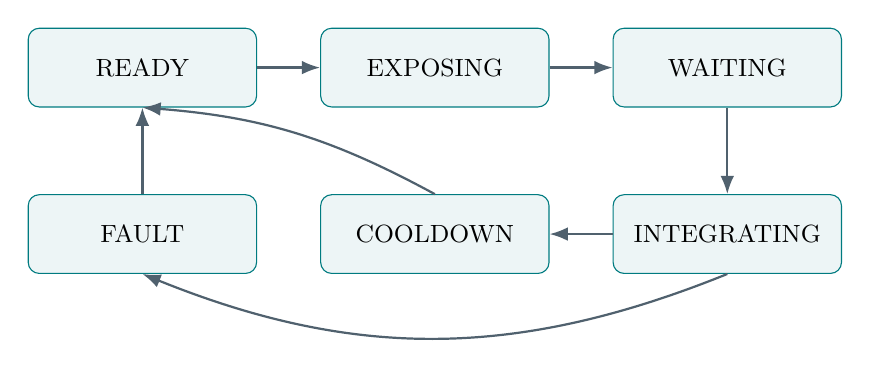
\begin{tikzpicture}[font=\small,box/.style={draw=accent,fill=pale,rounded corners,
minimum width=29mm,minimum height=10mm,align=center},arr/.style={-{Latex},color=muted,thick}]
\node[box] (ready) {READY};
\node[box,right=8mm of ready] (expose) {EXPOSING};
\node[box,right=8mm of expose] (wait) {WAITING};
\node[box,below=11mm of wait] (integrate) {INTEGRATING};
\node[box,left=8mm of integrate] (cool) {COOLDOWN};
\node[box,left=8mm of cool] (fault) {FAULT};
\draw[arr] (ready)--(expose);
\draw[arr] (expose)--(wait);
\draw[arr] (wait)--(integrate);
\draw[arr] (integrate)--(cool);
\draw[arr] (integrate.south) to[bend left=22] (fault.south);
\draw[arr] (cool.north) to[bend right=12] (ready.south);
\draw[arr] (fault)--(ready);
\end{tikzpicture}
\end{center}
Ein Receipt setzt WAITING auf INTEGRATING. Erst der
nachfolgende Integrationsübergang kann Evidenz erzeugen.
Fehler und Timeout führen nach ihrer Integration zu FAULT;
der Rückweg benötigt einen eigenen Recovery-Übergang.
Vor der ersten Bindung gilt UNBOUND, nach Stop STOPPED.
Eine noch nicht gestartete Exposition kann abgebrochen werden.

QUIESCENT und WAITING können gleichzeitig gelten: Ein bereits
angenommener Auftrag wird noch abgearbeitet, während neue
Expositionen gesperrt sind. Seine Antwort kann wegen der
geänderten Bindung als SUPERSEDED enden.

\nextsection{23 / AUSFÜHRBARE EXPOSITION}{Zwei Messorgane in einem endlichen Feld}
Das Testfeld besteht aus $n$ radialen Sektoren und jeweils $d$
geordneten Zellen. Eine Zelle $c_{s,j}$ trägt die booleschen
Eigenschaften \emph{solid} und \emph{beacon}. Das Standardfeld
hat $n=8$ und $d=4$; der Vertrag erlaubt $2\leq n\leq16$ und
$1\leq d\leq32$.

\begin{tabularx}{\linewidth}{@{}lY@{}}
\toprule
Organfrage & Messbedeutung\\\midrule
\texttt{ray\_clear} & Ist der gesamte gebundene Sektor frei von
einer soliden Zelle? Ein erstes Hindernis genügt als Gegenbeleg.\\
\texttt{beacon\_present} & Existiert mindestens ein Beacon im
endlichen Sektor? Die Beobachtung erreicht Zellen bis einschließlich
des ersten Hindernisses.\\
\bottomrule
\end{tabularx}

Für Clearance gilt
\[
q_{\rm clear}(s)=\neg\bigvee_{j=0}^{d-1}\mathrm{solid}(c_{s,j}).
\]
Für die Beaconfrage definiert der Evaluator die vollständige
Wahrheit durch $\bigvee_j\mathrm{beacon}(c_{s,j})$. Das
Messorgan erhält dagegen nur den erreichbaren Präfix.
Ein sichtbarer Beacon belegt true. Wird der ganze Sektor
ohne Beacon beobachtet, folgt false. Verbleibt hinter einem
Hindernis ein unbeobachteter Rest, lautet das Ergebnis OCCLUDED.
Ein Beacon auf der Hinderniszelle selbst zählt als sichtbar.

\subsection{Expositionswitness}
Der gewählte Sektor ist Teil der Fragenidentität:
\[
q=(\mathrm{organID},s),\qquad s\in\{0,\ldots,n-1\}.
\]
Ein Richtungswechsel überschreibt deshalb nicht die Bedeutung
eines bestehenden Facts. Der Witness bindet Frage, Sektorzahl,
fortlaufenden Schrittzähler, Zeitpunkt, StateRef sowie Ziel-
und Frameepoche. Bei Wechsel von $s$ nach $s'$ gilt
\[
u'=u+((s'-s)\bmod n),\qquad s'=u'\bmod n.
\]
Die Bewegungskonvention ist positiv zyklisch. Ein unveränderter
Sektor erzeugt keinen zusätzlichen Umlauf.

Der gestartete Worker erhält genau Query und Sektor dieser
Exposition und liest einen begrenzten JSON-Schnappschuss des
Felds. Die Messreferenz bindet dessen Digest. Dies realisiert
eine ausführbare diskrete Orientierung; Quaternionen,
720-Grad-Spinorsemantik und physischer Transport folgen daraus nicht.

\nextsection{24 / ORGANBANK}{Faire Abdeckung und reserviertes Messbudget}
Die Bank enthält zwei explizit konfigurierte Organe. Ein Worker
führt höchstens eine aktive Messfolge gleichzeitig aus.
Die vorhandene Parallelität betrifft HTTP-Annahme und
Darstellung; die Messungen selbst sind seriell geordnet.

\subsection{Drei festgelegte Expositionspolitiken}
\begin{tabularx}{\linewidth}{@{}lY@{}}
\toprule
Politik & Wahl im jeweils ausgewählten Organ\\\midrule
fixed & immer Sektor 0; Ablation ohne veränderliche Exposition.\\
uniform & deterministische Pseudozufallswahl aus der gebundenen
Seedfolge; wiederholte Sektoren sind möglich.\\
coverage & der am längsten nicht angefragte Sektor zuerst;
unbesuchte Sektoren besitzen Vorrang, stabile ID löst Gleichstand.\\
\bottomrule
\end{tabularx}
Zwischen ausführbaren Organen gewinnt das am längsten nicht
bediente Organ. Die Politik verwendet keine verborgenen
Weltwerte. Coverage ist eine endliche Abdeckungsheuristik;
sie maximiert keinen gemessenen Informationsgewinn und
verwendet das Navigationsziel nicht als Belohnungsfunktion.

\subsection{Budgetvertrag}
Für Kosten $c>0$, bisherige Ausgaben $B_{\rm used}$ und
aktuelles Limit $B_{\rm max}$ ist Dispatch nur zulässig, wenn
\[
B_{\rm used}+c\leq B_{\rm max}.
\]
Der Dispatch-Commit reserviert und verbraucht $c$ genau einmal.
Auch fehlgeschlagene oder später überholte Messungen behalten
ihre Kosten. Ein Budgetwechsel verlangt
$B'_{\rm max}\geq B_{\rm used}$. Er annulliert keine bereits
gebundenen Aufträge. Der Request enthält seine ursprüngliche
Budgetepoche; die Änderung des Limits wird separat protokolliert.

Im Vergleich kostet jede Messung eine abstrakte Einheit.
CPU-Zeit, mechanische Bewegung und physische Energie werden
damit nicht gemessen. Ein produktiver Kostenvertrag benötigt
diese Komponenten zusätzlich.

\subsection{Epochen und Integration}
Die Integration prüft Ziel- und Frameepoche erneut, auch wenn
das Receipt bereits eingetroffen ist. Eine inzwischen überholte
Bindung erzeugt SUPERSEDED und keinen Beobachtungsrecord.
Zeitüberschreitung bezieht sich auf den Eingang des Receipts:
Eine verspätete erfolgreiche Antwort wird zu TIMEOUT.

\nextsection{25 / SEGMENTIERTE LINEAGE}{Fortsetzung ohne Zustands- oder Budgetreset}
Das Organjournal besteht aus nummerierten JSONL-Segmenten.
Jeder Header bindet Konfiguration, Segmentindex,
globale Startsequenz, Anfangszustand und Kopf des Vorgängers.
Die erste Segmentbindung besitzt keinen Vorgänger.
Folgende Segmente dürfen nur nach Erreichen der festgelegten
Recordgrenze beginnen.

Die Rotation ändert weder Organidentitäten noch Evidenz,
Schrittzähler, Requestzähler oder Budget. Ihre Grenze ist eine
Speichergrenze, kein semantischer Neustart.
Die Hashverkettung setzt am neuen Segmentheader fort.
Replay prüft jedes Segment und führt alle Übergänge erneut aus.
Fehlende Segmente, falsche Anschlüsse und semantisch
manipulierte Records werden abgewiesen.

\subsection{Schreib- und Wiederanlaufvertrag}
Compute--Append--Flush--fsync--Publish bleibt erhalten.
Der Writer prüft zusätzlich Dateibindung und Schreibposition.
Ein unvollständiger letzter Record wird vor explizitem Resume
unverändert als Fragment gesichert. Ein unvollständiger neuer
Segmentheader wird ebenfalls gesichert; danach wird am
geprüften Vorgänger fortgesetzt. Eine vollständig korrupte
Zeile ist kein reparierbares Fragment.

Die Runtime setzt beim Wiederanlauf die logische Uhr auf
letzten Takt plus TTL plus eine Millisekunde. Alte Evidenz
verfällt, offene Requests werden aufgegeben, und die Organe
werden erneut an ihren Modellvertrag gebunden.
Eine laufende Session hat genau einen Writer. Gleichzeitige
Writer, externes Überschreiben aktiver Journale und eine
vertrauenswürdige Mehrbenutzer-Speicherung sind nicht implementiert.

\subsection{Entfernung redundanter Historienkopien}
Der ursprüngliche Kernel archiviert nach jedem inneren Ereignis
einen vollständigen Renderzustand. In der äußeren Organruntime
würde jede Kandidatenkopie diese ganze Archivfolge erneut
kopieren. Der neue OrganKernel behält Ereigniszählung,
Evidenz und innere Traces, entfernt aber dieses zweite
Snapshotarchiv. Das Segmentjournal bleibt die Replaygrundlage.

Ein Vergleich über 120 Ereignisse erzeugt dieselben
Kernzustände und inneren Tracedigests wie der vollständige
Interpreter. Innere Bundleexporte sind für diesen Modus
gesperrt; der zuständige Export ist Segment-Replay.
Historische Beobachtungen und Traces wachsen weiterhin.
Rotation bedeutet deshalb keine konstante Speichernutzung
oder konstante Wiederanlaufzeit.

\nextsection{26 / EXPOSITIONSVERGLEICH}{Vorab gebundener Versuch und Ergebnis}
Der Vergleichsvertrag wurde vor Erzeugung und Auswertung
der Fälle gespeichert. Zwölf Feldseeds definieren je ein
statisches Feld mit acht Sektoren und vier Zellen pro Sektor.
Alle drei Politiken erhalten dasselbe jeweilige Feld,
16 Messungen und Kosten von einer Einheit pro Messung.
TTL 100000\,ms und eine logische Versuchsuhr verhindern
hier Verfall während des Vergleichs.

Generator, Messfunktion und Evaluator besitzen getrennte
Programmfunktionen. Der Planner verwendet nur Deskriptoren,
seine Historie und Receipts. Diese Trennung ist keine
Sicherheitsisolation gegen einen absichtlich veränderten Planner.
Die Mess- und Wahrheitsfunktionen stammen aus demselben
endlichen Modell; der Versuch ist kein unabhängiger
Realweltbenchmark.

\begin{tabularx}{\linewidth}{@{}lrrr@{}}
\toprule
Politik & Fragen angefragt & Fragen Known & Falsche Known\\
& Mittel / 16 & Mittel / 16 & Anzahl / Known gesamt\\\midrule
fixed & 2,00 & 1,83 & 0 / 22\\
uniform & 10,00 & 8,67 & 0 / 104\\
coverage & 16,00 & 13,67 & 0 / 164\\
\bottomrule
\end{tabularx}

Die 36 Läufe umfassen 576 Messungen und lassen sich
vollständig reproduzieren. Die Zahlen zählen verschiedene
Fragen, nicht die Zahl positiver Umweltobjekte.
Angefragt bedeutet außerdem nicht automatisch bestimmt:
Eine verdeckte Beaconfrage bleibt Unknown.

\subsection{Interpretation}
Die feste Richtung misst bei zwei Organen nur zwei verschiedene
Fragen. Die systematische Politik erfasst bei 16 verfügbaren
Fragen und 16 Messungen jede Frage einmal. Dieser Vorteil
ist im statischen endlichen Modell strukturell zu erwarten.
Die gleichverteilte Politik verwendet einen gebundenen
Pseudozufallsgenerator und kann Fragen mehrfach auswählen.

Damit ist der Nutzen veränderlicher Exposition gegenüber
der festen Richtung konkret nachgewiesen. Daraus folgt
keine Überlegenheit gegenüber optimierten Scanverfahren,
aktiver Inferenz oder realen Sensorsystemen. Der Versuch
misst weder Laufzeit noch Latenz. Null beobachtete Fehler
bei den genannten Fallzahlen beweisen keine universelle Fehlerfreiheit.

\begin{lstlisting}
ProtocolDigest
81d25230ec8f1fb7b6b8e73d652629c185d258822463a6b77797f78bd2e0b700
\end{lstlisting}

\nextsection{27 / ORGANINTEGRATION}{Messprozesse, HTTP und Fehlerbehandlung}
Der Integrationslauf startet die feste Messfunktion tatsächlich
in Unterprozessen. Das Harness verändert ausschließlich sein
selbst erzeugtes synthetisches Feld. Die Runtime erhält
Messantworten und Steuerereignisse; die Darstellung erhält
Maschinenprojektionen über einen lokalen HTTP-Dienst.

\begin{tabularx}{\linewidth}{@{}rrY@{}}
\toprule
Sequenz & Requests & Erreichter Zustand\\\midrule
122 & 16 & erster vollständiger Sektorzyklus; 15 bestimmte Fragen,
eine Beaconfrage bleibt wegen Verdeckung offen.\\
136 & 18 & neu eingefügtes Hindernis erkannt; Clearance S0 false.\\
248 & 34 & Entfernung des Hindernisses erkannt; Clearance S0 true.\\
320 & 34 & ruhende Bank; sämtliche Evidenz abgelaufen.\\
431 & 50 & automatische Wiedererfassung nach Ende der Pause.\\
439 & 51 & Epochenwechsel verwirft die alte Requestbindung.\\
446 & 52 & blockierter Prozess beendet; FAULT und Unknown.\\
453 & 53 & Recovery und nächste verwertbare Messung.\\
460 & 53 & Budget auf bereits verbrauchten Betrag begrenzt;
kein weiterer Dispatch.\\
473 & 55 & Erweiterung um zwei Einheiten genau verbraucht.\\
474 & 55 & Organe RETIRED; Endzustand und Checkpoint geprüft.\\
\bottomrule
\end{tabularx}

Die Transportantworten enthalten 50 OK, vier OCCLUDED
und einen tatsächlich ausgelösten Prozess-Timeout.
Eine transportseitig erfolgreiche Antwort kann bei Integration
wegen ihrer Epoche als SUPERSEDED enden.
Der Stop-Snapshot enthält 13 bestimmte Fragen: Er ist ein
historischer Endzustand, keine Behauptung dauernder Frische.

354 über HTTP gelieferte Projektionen wurden gegen den
Runtimezustand geprüft. Das Journal umfasst 15 Segmente.
Vollständiges Replay ergibt den StateDigest:
\begin{lstlisting}
2c815aab5d20411e491d3843c3af2049c7863b1e29040f8d1ec31e6f06e83c50
\end{lstlisting}
Ein neuer realer Durchlauf besitzt andere Zeitwerte und Digests.
Die aufgezeichnete Folge bleibt dagegen exakt reproduzierbar.
Die Phasenzeiten im JSON-Bericht sind Laufzeiten dieser
Ausführung, keine separat gemessenen Detektionslatenzen.

\nextsection{28 / BETRIEBSREICHWEITE}{Ausführbares Profil und offene Grenzen}
Das Organprofil startet standardmäßig mit acht Sektoren,
32 Budgeteinheiten, TTL 2000\,ms, Timeout 500\,ms,
Cooldown 50\,ms und einer nominellen Zykluspause von 40\,ms.
Der Standardlauf dauert höchstens 30 Sekunden.
64 Records bilden ein Segment; maximal 1024 Segmente und
10000 Sessionübergänge sind konfiguriert.
Die zuerst erreichte Grenze bestimmt den geordneten Stop.

Der Zeitschritt des Workers umfasst zusätzliche Rechen-,
Schreib- und Messzeit. Ein laufender Unterprozess begrenzt
die Reaktion auf Steuerbefehle bis zu Antwort oder Timeout.
Eine harte Echtzeitgarantie ist nicht gegeben.
Ein ausgeschöpftes Messbudget hält neue Aufträge an;
Ticks und Evidenzverfall laufen weiter. Das Live-Cockpit
kann das Limit durch einen protokollierten Auftrag erhöhen.

\begin{tabularx}{\linewidth}{@{}lY@{}}
\toprule
Vorhanden & Reichweite\\\midrule
Organidentität & zwei konfigurierte Organe; kein dynamisches Laden
beliebiger Programme über HTTP.\\
Kalibrierung & geprüfter idealer Modellvertrag; keine Messung
physischer Bias- oder Driftparameter.\\
Rotorparameter & diskreter Sektor und positiver Umlaufzähler;
kein kontinuierlicher räumlicher Träger.\\
Karte & deklarierte Ring- und Querbeziehungen zwischen Fragen;
keine rekonstruierte Umwelttopologie.\\
Ledger & appendierende Segmente und vollständige Reausführung;
keine Sensorbeglaubigung oder signierte externe Zeitbasis.\\
Ansicht & Live-/Replayprojektion mit Mess- und Herkunftsdetails;
keine metrische Registrierung oder XR.\\
\bottomrule
\end{tabularx}

Für die kompatiblen Profile bestehen 97 Python-Tests und
26 JavaScript-Prüfungen. Die Kartenstufe ergänzt diese in Kapitel 33.
Die JavaScript-Suiten verwenden eine minimale DOM-Umgebung.
Eine visuelle Prüfung in einem echten Browser war nicht
verfügbar. Die PDF wurde separat gerendert und auf Layout
geprüft; daraus folgt kein Browser- oder Carrierbenchmark.

\nextsection{29 / MESSFENSTER}{Typisierte lokale Kartenstücke}
Das Atlasprofil \texttt{grfps-witnessed-atlas/0.4.0} konkretisiert
K05--K07 und den Map-Lifecycle aus Anhang H.3 der Ausgangsschrift.
Sein Vertrag ist endlich: ganzzahlige zweidimensionale Punkte,
Rotationen um Vielfache von $90^\circ$ und ganzzahlige Translationen.
Identitäten gemeinsamer Landmarken werden vom Sensor vorgegeben.
Die Implementierung erkennt keine Landmarken aus Bildern.

Die booleschen Kernprofile behalten ihre deklarierten Graphkanten.
Der neue Mapper besitzt einen eigenen Ereignistyp für Punkt- und
Beziehungsdaten. Ein lokaler Patch wird nicht in einen booleschen
Messwert kodiert. Auch das neue Kartenjournal hat eine eigene
Profilkennung und semantische Replayprüfung.

\subsection{Auftrag und Patchvertrag}
Ein Auftrag bindet Fenster-ID, Quelle, Frame-Epoche, Auftrags-ID,
Ausgabezeit und Frist. Sein Expositionshash bindet diese Felder.
Bereits die Annahme kostet eine Budgeteinheit. Es darf genau ein
Auftrag offen sein; fehlgeschlagene oder überholte Aufträge geben
keine Kosten zurück.

Ein Patch bindet zusätzlich Abtastzeit, Messquellenhash, lokale
Landmarkenkoordinaten, explizit beobachtete Beziehungen und offene
Randlandmarken. Die Eingabeprüfung verlangt eindeutige IDs,
verschiedene Punktpositionen und höchstens eine boolesche Aussage
pro ungeordnetem Landmarkenpaar. Nicht beobachtete Paare besitzen
keinen stillschweigend negativen Wert.

\begin{lstlisting}
request -> patch | fail
retract(patch_id)
tick(at)
frame(at)
\end{lstlisting}
Ein akzeptierter Patch muss zum offenen Auftrag passen. Zukünftige
Abtastzeiten und doppelte Antworten werden zurückgewiesen. Eine
Antwort nach der logischen Frist erzeugt TIMEOUT; eine Antwort aus
einer inzwischen verlassenen Epoche erzeugt SUPERSEDED. Beide
integrieren keine Karte. Zeitfortschritt allein erzeugt keinen Patch.

\subsection{Ausführbarer Sensor}
\texttt{map\_worker.py} liest ein endliches synthetisches Weltmodell
in einem eigenen Prozess. Das gewählte Fenster bestimmt die sichtbaren
Landmarken und Beziehungen. Seine lokale Pose wird vor der Ausgabe
invertiert; der Mapper erhält diese Pose nicht. Der Adapter hat
keinen Schreibpfad in die Weltdatei. Nur der Versuchsharness ändert
seine eigene Fixture für den Gegenbelegversuch.

\nextsection{30 / OVERLAP-WITNESS}{Exakter Anschluss und globale Konsistenz}
Seien $P_i,P_j$ zwei aktuell gültige Patches und
$S_{ij}$ ihre gemeinsamen Landmarken-IDs. Ein Anschluss benötigt
mindestens zwei verschiedene gemeinsame Punkte und genau eine
Transformation
\[
T_{ij}(x)=R_r x+t,\qquad r\in\{0,1,2,3\},\quad t\in\mathbb Z^2,
\]
welche \emph{alle} gemeinsamen Punkte aufeinander abbildet.
Zudem dürfen gemeinsam beobachtete Beziehungen nicht widersprechen.
Ein gemeinsamer Punkt allein liefert GAP. Unvereinbare Geometrie
oder Gegenbelege liefern CONFLICT. Spiegelungen sind nicht zugelassen.
Es gibt weder numerisches Fitting noch eine implizite Toleranz.

\contract{GLUED ist eine abgeleitete, widerrufbare Entscheidung.
Ein Hash ist eine Inhaltsbindung und kein geometrischer Beweis;
die Kompatibilitätsprüfung muss tatsächlich ausgeführt werden.}

Der Witness enthält beide Patchhashes, gemeinsame IDs,
Transformation und das Minimum beider Ablaufzeiten. Sein eigener
Hash erlaubt eine eindeutige Referenz. \texttt{mapping.py} berechnet
die Entscheidung deterministisch aus den gültigen Patches neu.

\subsection{Mehrere Kartenstücke}
Paarweise passende Transformationen müssen auch im Zusammenhang
passen. Pro Komponente wird der lexikografisch erste Patch zum
lokalen Ursprung. Entlang der Anschlüsse werden Posen komponiert;
jeder weitere Pfad muss dieselbe Pose ergeben. Gleich benannte
Landmarken müssen komponentenweit denselben Ort besitzen.
Auch ein direkter Beziehungskonflikt darf nicht durch einen Umweg
über ein drittes Fenster verdeckt werden.

Bei einer solchen Inkonsistenz werden die beteiligten Anschlüsse
der gesamten Komponente quarantänisiert und die Patches getrennt
projiziert. Das ist eine bewusst konservative Regel. Sie ermittelt
keine minimale Menge schuldiger Kanten. Unabhängige Komponenten
werden davon nicht betroffen.

\subsection{Beziehungen und Koordinaten sind getrennte Aussagen}
Beziehungen tragen alle aktuell gültigen Patchreferenzen. Stimmen
sie überein, ist die Beziehung Known, gegebenenfalls mit Wert false.
Widersprechen sie, ist sie Ambiguous und ihr Wert bleibt unbestimmt.
Eine positive Beziehung ist noch keine globale Pose. Getrennte
Komponenten bleiben getrennte Karten; es wird keine Position
zwischen ihnen erfunden.

\nextsection{31 / REVALIDIERUNG}{Rücknahme, Ablauf und Framebindung}
Ein Patch $P$ ist zum Zeitpunkt $t$ genau dann aktiv, wenn er nicht
zurückgenommen wurde, seine Epoche der aktuellen Epoche entspricht
und $t<P.\mathrm{sampled\_at}+\mathrm{TTL}$ gilt. Bereits am exakten
Ablaufzeitpunkt ist er inaktiv. Das Journal behält seine Provenienz.

Jede Zustandsprojektion leitet Patches, Overlaps, Komponenten und
Beziehungen erneut ab. Entfällt eine Voraussetzung, verschwindet
ihr Anschluss. Ein Ersatzpatch löscht einen alten Beleg nicht
stillschweigend: Im Versuch wird der alte Patch explizit zurückgenommen.
Gleichzeitig gültige gegensätzliche Belege bleiben widersprüchlich.

\subsection{Journal und Veröffentlichung}
Der Reducer prüft zuerst auf einer Kopie. Das Journal schreibt
anschließend den vollständigen Übergang mit Vorzustand, Nachzustand,
Ausgabe und Vorgängerhash. Erst nach Flush und fsync wird der neue
Zustand veröffentlicht. Ein Schreibfehler sperrt weitere Schreibversuche
dieses Writers. Das Replay führt alle Ereignisse erneut aus und
vergleicht kanonische Bytes, nicht lediglich gespeicherte Hashketten.

Der Atlaswriter prüft Dateidentität und Dateigröße. Er bietet keine
Mehrschreiberkoordination. Unvollständige letzte Records werden
abgewiesen; automatische Tailreparatur und Fortsetzung sind im neuen
Atlasprofil nicht implementiert. Die segmentierte Wiederaufnahme
bleibt eine Fähigkeit des getrennten Organprofils 0.3.0.

\subsection{Grenzen des endlichen Vertrags}
Die Standardkonfiguration erlaubt 16 Aufträge, 512 Ereignisse,
32 archivierte Patches, 32 Punkte und 128 Beziehungen pro Patch.
Die TTL beträgt 100 logische Millisekunden, die Auftragsfrist 20.
Ein Record ist auf 256 KiB begrenzt. Patches werden nicht dauerhaft
kompaktiert; ausgeschöpfte Kapazität beendet weitere Aufnahmen.
Die Paarprüfung wächst quadratisch mit der Patchzahl.

Der Prozessadapter besitzt zusätzlich einen realen Timeout von zwei
Sekunden. Ein Prozessfehler oder dieser externe Timeout wird als
ERROR in den logischen Versuch aufgenommen. Logische Messzeit und
verstrichene Prozesszeit sind ausdrücklich verschiedene Größen.
Die Ausführung ist kein Echtzeit- oder Latenzbenchmark.

\nextsection{32 / KARTENVERSUCH}{Acht Messprozesse und reversible Anschlüsse}
Das Protokoll wird vor der ersten Aufnahme gespeichert. Die Ausgangswelt
hat sechs Landmarken, vier positive und zwei explizit negative
Beziehungen. Die beiden ersten Fenster teilen zwei Landmarken;
das dritte Fenster hat keinen gemeinsamen Bezug zu ihnen.
Weltkoordinaten und Fensterposen bleiben außerhalb des Reducers
und der Ansicht. Die Fixture ist eine Modellreferenz, keine
unabhängige empirische Datenquelle.

\begin{center}\begin{tabular}{@{}lrrr@{}}\toprule
Zustand & Sequenz & Anschlüsse & Konflikte\\\midrule
Erstes Fenster & 2 & 0 & 0\\
Zweites Fenster & 4 & 1 & 0\\
Getrenntes drittes Fenster & 6 & 1 & 0\\
Alter Beleg zurückgenommen & 7 & 0 & 0\\
Gegenbeleg aufgenommen & 9 & 0 & 1\\
Konsistenter Ersatz & 12 & 1 & 0\\
Gemeinsamer Witness abgelaufen & 13 & 0 & 0\\
Framewechsel & 14 & 0 & 0\\
Neue Aufnahmen im neuen Frame & 18 & 1 & 0\\
Überholte Antwort unterdrückt & 21 & 0 & 0\\
Abschließender Takt & 22 & 0 & 0\\\bottomrule
\end{tabular}\end{center}

Nach den ersten drei Aufnahmen rekonstruiert das Modell alle vier
positiven Beziehungen ohne zusätzliche positive Kante. Der vorab
festgelegte deklarierte Kontrollgraph enthält dieselben vier positiven
Beziehungen und zwei unbelegte zusätzliche Kanten.
\begin{center}\begin{tabular}{@{}lrrr@{}}\toprule
Graph & Richtig positiv & Falsch positiv & Fehlend\\\midrule
Deklarierte Kontrolle & 4 & 2 & 0\\
Gemessene Beziehungen & 4 & 0 & 0\\\bottomrule
\end{tabular}\end{center}
Die Messvariante benötigt dafür drei Fensteraufnahmen. Die deklarierte
Kontrolle führt keine Sensorabfrage aus. Dies ist ein konstruiertes
Konformitätsbeispiel mit absichtlich fehlerhaftem Kontrollgraphen,
kein fairer Leistungsnachweis gegenüber einem Mappingverfahren.
Der vollständige Fehler- und Erneuerungslauf verbraucht acht Aufträge.

\nextsection{33 / SECOND-LAYER-ANSICHT}{Replay, Evidenz und Verifikation}
Die Datei \texttt{map\_demo.html} zeigt im Profil 0.4.0 23 Zustände einschließlich des
Initialzustands. Der Zeitschieber wählt die zugehörigen 22 Ereignisse.
Jede Kartenkomponente besitzt eigene Koordinaten; ihre Anordnung
auf dem Bildschirm hat keine räumliche Bedeutung zwischen Komponenten.
Offene Randpunkte, bekannte negative Beziehungen und Widersprüche
haben getrennte sichtbare Markierungen.

Die Ansicht enthält keine verborgenen Weltkoordinaten und keine
Evaluatorwahrheit. Sichtbar sind Maschinenprojektion, lokale Patches,
Beziehungsbelege, Overlap-Witnesses und inaktive Patchgründe. Sie
stellt den aufgezeichneten Lauf dar. Eine laufende HTTP-Kartenaufnahme
oder automatische Messwahl ist im Profil 0.4.0 noch nicht enthalten;
das aktive Profil ab Kapitel 34 ergänzt diese Rollen.
Die vorhandene Organ-Liveansicht bleibt als \texttt{organ\_demo.html}
und über \texttt{start.py} verfügbar.

\subsection{Prüfumfang}
22 neue Python-Tests prüfen unter anderem Vierteldrehungen,
Spiegelungskonflikte, unzureichenden Overlap, Zyklusinkonsistenz,
Konfliktumgehung, Fristen, Budget, Framewechsel, Ablauf,
Rücknahme, Prozessausführung, Schreibfehler und semantische
Replaymanipulation. Zusammen mit den erhaltenen Profilen sind es
119 Python-Tests. Zehn neue JavaScript-Prüfungen ergänzen die
bisherigen 26 Prüfungen. Sie führen das echte Ansichtsskript mit
einem minimalen DOM aus; eine visuelle Browserprüfung war nicht verfügbar.

Der Releaseprüfer berechnet alle Kartenrecords neu, prüft jeden
Patch gegen seine archivierte Weltfixture und berechnet die
Kontrollgraphmetriken erneut. Zusätzlich werden die vorhandenen
Datei- und Organjournale sowie die 36 Expositionsversuche erneut geprüft.

Kartenjournal, finaler Head:
\begin{lstlisting}
6a008fcd268c4b14f3c0095eb00249ad701eadeda11090a60144b7ee290ff725
\end{lstlisting}
Finaler Zustandsdigest:
\begin{lstlisting}
09c69ced853432161a345edae11bb11246b12ebac4427cb0a404a838c750b35a
\end{lstlisting}

\nextsection{34 / AKTIVES FENSTERORGAN}{Randbelege werden zu Folgeaufträgen}
Das Profil \texttt{grfps-active-atlas/0.5.0} setzt die Kartenstufe
in einen laufenden Regelkreis. Der äußere Reducer enthält den
unveränderten Atlasreducer. Ein Aufnahmeorgan besitzt die Zustände
READY, WAITING, QUIESCENT und STOPPED. Seine Exposition ist die
gewählte Fenster-ID; sein Ergebnis ist ein typisierter Patch.

Die neue Session verwendet die lokale HTTP-Infrastruktur der
vorhandenen Runtime. Sie übernimmt deren Prinzip eines einzigen
Zustandsbesitzers und eines begrenzten Kontrollkanals. Die
booleschen Feldorgane werden nicht in diese Session hineinkopiert;
eine gemischte Organbank bleibt eine weitere Integrationsaufgabe.

\subsection{Gebundener Abfragekatalog}
Ein Katalog benennt ausführbare Fenster und ihre bekannten
Einstiegslandmarken. Genau ein Fenster ist ohne Einstieg zulässig:
der Bootstrap. Jedes weitere Fenster benötigt mindestens zwei
gebundene IDs. Für einen Folgeauftrag müssen alle seine Einstiegs-IDs
aktuell beobachtet sein; mindestens eine davon muss in einem
beobachteten offenen Rand vorkommen.

Der Katalog enthält keine Koordinaten, Fensterpose, versteckten
Beziehungswerte oder Aussage, dass die Abfrage erfolgreich sein wird.
Er ist dennoch Vorwissen über verfügbare Abfragen. Die Steuerung
entdeckt keine beliebigen unbekannten Sensorpositionen. Ein zulässiger
Auftrag ist ein Versuch, eine offene Grenze zu untersuchen; er garantiert
keinen kompatiblen Overlap.

\subsection{Deterministische Auswahl}
Unter den zulässigen Fenstern werden zuerst noch nie versuchte
Fenster gewählt. Danach entscheidet die älteste Versuchsuhr;
gleiche Prioritäten werden über die Fenster-ID aufgelöst. Erneute
Versuche sind frühestens nach dem gebundenen Refreshintervall erlaubt.
Das verhindert eine unmittelbare Fehlerschleife und erlaubt späteres
Erneuern alter Aussagen. Die Standardwerte sind 700 ms Refresh,
1500 ms TTL und 600 ms Auftragsfrist.

Der Vorschlag bindet Fenster, Grund, Einstiegs-IDs, Patchreferenzen
und Frame. Bei Dispatch werden Zeit und Evidenz erneut ausgewertet;
der übergebene Vorschlag muss bytegenau dem aktuellen Vorschlag
entsprechen. Erst dann wird eine Budgeteinheit reserviert.
Es gibt genau einen offenen Messauftrag.

\nextsection{35 / LAUFENDER BETRIEB}{Nebenläufiger Sensor und unmittelbare Projektion}
Der Zustandsbesitzer arbeitet in kurzen Zyklen. Ein einzelner
Worker-Thread beaufsichtigt den festen Sensorprozess. Während der
Prozess läuft, verarbeitet der Besitzer weiter Kontrollbefehle und
Zeitfortschritt. Dadurch können Aussagen ablaufen und Pause kann
wirksam werden, ohne auf das Messende zu warten.

Der Worker liest die eigene synthetische Weltdatei und bestimmt den
Abtastzeitpunkt über die gemeinsame monotone Rechneruhr. Der Adapter
begrenzt den Prozess auf die verbleibende Auftragsfrist. Ein Timeout
beendet den Prozess und liefert eine explizite Fehlerantwort.
Ein fehlerhaftes Protokoll wird nicht als Patch integriert.

\subsection{Pause, Frame und Stop}
Beim Eintritt in Pause wird die Frame-Epoche erhöht. Diese konservative
Regel entzieht allen bisherigen Patches sofort ihre operative Gültigkeit.
Eine noch laufende Antwort gehört zur alten Epoche und wird unterdrückt.
Pause erstattet keine Messkosten. Erneute Freigabe lässt nur neue
Aufträge und neu gebundene Evidenz zu.

Stop sperrt neue Aufträge und wartet die endliche Restfrist des offenen
Auftrags ab. Erst nach dessen Abschluss wird STOPPED protokolliert.
Ein Stop nimmt bereits integrierte Evidenz nicht automatisch zurück;
ihre zeitliche Gültigkeit bleibt ein separater Vertrag.

\subsection{Live-Ansicht}
Die Live-Ansicht fragt alle 250 ms den aktuellen vollständigen Snapshot
ab. Sie zeigt Kartenkomponenten, Beziehungen, Konflikte, Organstatus,
Pause und den nächsten evidenzgebundenen Vorschlag. Die Kontrollen
Pause, Weiter messen, Frame erneuern und Stop gelangen über eine
auf 16 Einträge begrenzte Queue zum Zustandsbesitzer.

Die API bleibt an Loopback gebunden und prüft Host sowie Origin wie
die vorhandene Infrastruktur. Eine angenommene HTTP-Anfrage bestätigt
die Aufnahme in die Queue. Sie ist noch keine Bestätigung einer
abgeschlossenen Messung. Verbindungsfehler markieren die Ansicht
explizit als nicht aktuell.

Die Kartenprojektion verwendet in dieser Version vollständige Resets,
keine inkrementellen Kartendeltas. Der Browser hält im Live-Modus nur
den neuesten Zustand. Die Dateireplay-Ansicht bleibt ohne Netzwerkaktivität.

\nextsection{36 / WIEDERANLAUF}{Budgeterhalt und erneute Framebindung}
Das aktive Journal bindet die gesamte äußere Session einschließlich
Abfragekatalog, Versuchszeiten, Pause, Phase und innerem Atlaszustand.
Vor- und Nachzustände werden bei jeder Wiederaufnahme vollständig
rekonstruiert. Die Hashdomäne enthält die neue Profilkennung.
Die Append-first-Regel und die Veröffentlichung nach fsync bleiben erhalten.

Beim Wiederanlauf wird die Frame-Epoche erhöht. Ein nach einem
Abbruch noch offener Auftrag wird als Fehler abgeschlossen. Seine
Kosten und Auftrags-ID bleiben verbraucht. Der CLI-Start setzt die
logische Uhr konservativ hinter die alte Uhr plus TTL; dies behauptet
keine Messung der tatsächlichen Ausfallzeit. Alte Evidenz wird dadurch
nicht irrtümlich frisch weiterverwendet.

\contract{Wiederaufnahme setzt Budget, Auftragszähler, Versuchszeiten
und Journalgeschichte nicht zurück. Sie erzeugt eine neue operative
Framebindung innerhalb derselben aufgezeichneten Session.}

\subsection{Kapazität und Fehlergrenze}
Der Standardvertrag enthält 1024 äußere Ereignisse und 4096 innere
Atlasereignisse. Vier äußere Plätze werden für den geordneten Abschluss
reserviert. Das bestehende Archivlimit von 32 Patches bleibt bestehen.
Bei ausgeschöpftem Messbudget entstehen keine weiteren Aufträge;
die Zeit- und Kontrollverarbeitung kann bis zum Ereignislimit fortlaufen.

Die neue Wiederaufnahme akzeptiert ausschließlich vollständige,
semantisch valide Journale. Beschädigte oder unvollständige letzte
Records werden abgewiesen. Es gibt weder automatische Tailreparatur
noch eine Mehrschreibersperre. Ein gleichzeitiger zweiter Writer ist
kein unterstützter Betriebsmodus. Langzeitkompaktion und unbegrenzter
Dauerbetrieb bleiben offen.

\nextsection{37 / AKTIVER NACHWEIS}{Automatische Expansion, Pause und Fortsetzung}
Der Integrationsharness startet die echte lokale HTTP-Schnittstelle
und echte nebenläufig beaufsichtigte Sensorprozesse. Die Testwelt
enthält zusätzlich ein Brückenfenster. Dieses wird erst nach den
beobachteten Einstiegslandmarken des rechten Fensters zulässig;
anschließend wird die bisher getrennte Insel erreichbar.

\begin{center}\begin{tabular}{@{}lrrr@{}}\toprule
Zustand & Sequenz & Verbrauch & Anschlüsse\\\midrule
Vier Fenster erschlossen & 17 & 4 & 3\\
Pause aktiv & 19 & 4 & 0\\
Pause über TTL gehalten & 91 & 4 & 0\\
Vier Fenster neu aufgenommen & 109 & 8 & 3\\
Geordnet gestoppt & 110 & 8 & 3\\
Nach Wiederanlauf beendet & 129 & 12 & 3\\\bottomrule
\end{tabular}\end{center}

Der Lauf enthält 92 erfolgreiche Vergleiche zwischen der tatsächlich
über HTTP empfangenen Projektion und dem Maschinenzustand. Beim
Wiederanlauf bleiben die zuvor verbrauchten acht Einheiten erhalten.
Der gesamte Lauf erreicht das vorab gebundene Budget von zwölf.
Die konkreten Sequenzzahlen hängen von Prozesslaufzeiten ab;
der gespeicherte Ereignisstrom wird dagegen deterministisch reproduziert.

19 neue Python-Tests prüfen unter anderem Vorschlagsbindung,
Ablauf zwischen Vorschlag und Dispatch, Kataloggrenzen, Gegenbelege,
Budgeterhalt, Schreibfehler, Replaymanipulation, geordneten Kapazitätsstop,
einen tatsächlich blockierten und abgebrochenen Prozess sowie Pause
bei laufendem Worker. Acht neue JavaScript-Prüfungen ergänzen
Offlineverhalten, Vorschlagsanzeige, Pause und veraltete Projektionen.
Insgesamt bestehen 138 Python-Tests und 44 JavaScript-Prüfungen.
Eine visuelle Browserprüfung war nicht verfügbar; die Ansichtslogik
wurde mit minimalem DOM ausgeführt. Die PDF wurde gerendert geprüft.

Finaler Journalhead:
\begin{lstlisting}
75b19baf2379c48c2eb4ae7649e1684b8e67e5d003413efb8cc8703dd9443b73
\end{lstlisting}
Finaler Zustandsdigest:
\begin{lstlisting}
95fe0e84cb82457c7271dd8cff4977f4dd2480504ab46b1874114f07b21d7df4
\end{lstlisting}

\nextsection{38 / GEMISCHTE ORGANBANK}{Drei Organe unter einem Budget}
Das Profil \texttt{grfps-organ-bank/0.6.0} enthält ein Fensterorgan
und die beiden vorhandenen Feldoperatoren \texttt{ray\_clear} und
\texttt{beacon\_present}. Der Fensterpfad verwendet den aktiven
Atlasreducer. Die Feldpfade verwenden den vorhandenen
\texttt{FieldRunner} und den festen Feldworker aus Profil 0.3.0.
Die Aufnahmeverwaltung erfolgt jetzt über eine gemeinsame Session.

\begin{center}\begin{tabular}{@{}llr@{}}\toprule
Organ & Antworttyp & Standardkosten\\\midrule
Fenster & Patch & 2\\
Freie Sicht & BooleanEvidence & 1\\
Beacon-Präsenz & BooleanEvidence & 1\\\bottomrule
\end{tabular}\end{center}

Die Kosten werden beim Dispatch reserviert. Zulässig ist ein Auftrag
nur dann, wenn das kumulativ verbrauchte Budget einschließlich seiner
Kosten innerhalb des gemeinsamen Limits bleibt. Fehlende, abgebrochene
und überholte Antworten geben keine Kosten zurück. Ein Fensterauftrag
kann bei einer verbleibenden Einheit nicht mehr angenommen werden;
eine zulässige boolesche Abfrage kann diese Einheit noch verwenden.

\subsection{Auswahl und Typbindung}
Die Fensterkandidaten entstehen unverändert aus den aktuellen
Randbelegen und dem Katalog. Jedes Feldorgan wählt seinen ältesten
beziehungsweise noch nicht abgefragten Sektor. Unter den bezahlbaren
Organvorschlägen entscheidet der älteste Dispatchzähler; Gleichstände
werden über die Organ-ID aufgelöst. Diese endliche Auswahlregel
optimiert keinen behaupteten Informationsgewinn.

Ein Bankauftrag bindet globale ID, Organ, Kosten, Frame, Ausgabezeit,
Frist und typisierte Nutzlast. Sein Expositionsdigest bindet sämtliche
Felder. Der Fensterauftrag enthält zusätzlich den inneren Atlasauftrag.
Es gibt bankweit genau einen offenen Auftrag. Ein Patch kann keine
boolesche Antwort ersetzen; eine boolesche Antwort kann keine Karte
anlegen. Die Zuordnung wird vor der Zustandsänderung geprüft.

Der bisherige vollständige Mikroautomat der separaten Organruntime
wird nicht unverändert als zweite Verwaltungsebene mitgeführt.
Die Bank integriert dessen Messoperatoren und Prozessadapter unter
einem gemeinsamen, eigenen Aufnahmevertrag. Beide Profile bleiben
für ihren jeweiligen Vertrag ausführbar.

\nextsection{39 / TYPISIERTE EVIDENZ}{Feldwahrnehmung und Karte bleiben unterscheidbar}
Die booleschen Feldorgane behalten ihre ideale Messsemantik:
Freie Sicht prüft den endlichen Strahl; Beacon-Präsenz kann hinter
einem Hindernis einen verdeckten Rest besitzen. Ein solcher Rest
liefert OCCLUDED mit unbestimmtem Wert. Er ist keine negative
Aussage. Ein bekannter negativer Wert benötigt eine erfolgreiche
explizit boolesche Antwort.

Pro Kombination aus Feldorgan und Sektor wird der zuletzt akzeptierte
Beleg gehalten. Er bindet Auftrags-ID, Frage, Sektor, Frame,
Abtastzeit, Ergebnis und Messquellenhash. Beim Ersetzen wandert der
vorherige Beleg in das geprüfte Archiv. Zeitfortschritt und Framewechsel
entziehen alter Evidenz ihre operative Gültigkeit.

\subsection{Fehler- und Quellenvertrag}
Antworten mit falschem Typ, falscher Exposition, zukünftiger Abtastzeit
oder ungültiger Nutzlast werden abgewiesen. Ein Prozessfehler erzeugt
keine neue Wahrheitsaussage. Ein zuvor gültiger Beleg kann bis zu seinem
Ablauf bestehen bleiben; der Fehler wird zusätzlich als Ergebnis des
fehlgeschlagenen Auftrags sichtbar.

Die beiden Weltdateien sind synthetische Fixtures. Dass sie getrennt
abgefragt werden, begründet keine statistische Quellenunabhängigkeit.
Es findet keine Evidenzfusion zwischen Feldwerten und Kartenbeziehungen
statt. Eine bekannte freie Sicht wird nicht automatisch zu einer
Kartenkante. Dafür wäre ein zusätzlicher geprüfter Domänenvertrag nötig.

\subsection{Bankprojektion}
Die Ansicht enthält neben dem Atlas eine Tabelle der Feldfragen,
der Antworttypen und der Kosten. Known false, Unknown und beobachtete
Verdeckung bleiben getrennt. Der globale Verbrauch wird unabhängig
von den inneren Fensterzählern angezeigt. Ein Archivfeld zeigt die
Anzahl residenter und bereits zurückgelegter Belege sowie die
aktuelle Inhaltsbindung des Archivs.

Pause, Framewechsel, Stop und Wiederaufnahme gelten bankweit.
Pause invalidiert konservativ die alte Framebindung. Ein bei Pause
noch offener Auftrag behält seine Kosten; seine überholte Antwort
kann keine neue operative Evidenz erzeugen.

\nextsection{40 / ARCHIVGRENZE}{Inaktive Belege aus dem Arbeitsspeicher lösen}
Die Verdichtung entfernt ausschließlich Belege, die bereits außerhalb
des aktuellen Gültigkeitsvertrags liegen. Für Patches gelten die
vorhandenen Gründe Ablauf, Rücknahme oder alte Framebindung.
Boolesche Belege werden bei Ablauf, Framewechsel oder Ersetzung
archiviert. Aktive Patches dürfen nicht zurückgelegt werden.

Ein Compact-Ereignis bindet die vollständige sortierte Menge der
zu diesem Zeitpunkt entfernbaren Einträge. Die Maschine berechnet
diese Menge erneut und verlangt kanonische Bytegleichheit. Ein
unvollständiger, veralteter oder manipulierter Vorschlag wird abgewiesen.

\subsection{Archivkette und vollständiger Inhalt}
Jeder Archivrecord enthält Typ, ID, Inhaltsreferenz, vollständigen
Beleg, Vorgängerdigest und fortlaufenden Archivindex. Der neue
Archivdigest bindet diesen Record. Die Records werden als Ausgabe
des semantisch geprüften Journalübergangs geschrieben. Erst nach
erfolgreichem Flush und fsync wird der Zustand mit entfernter
Residentkopie veröffentlicht.

\[
A_{n+1}=H(\mathrm{profile},\mathrm{ArchiveEntry},
           n,A_n,\mathrm{type},\mathrm{id},\mathrm{ref},\mathrm{value}).
\]
Die operative Maschine hält danach nur Zähler und Kettenkopf,
zusätzlich zu den noch residenten Belegen. Die letzte Ereignisausgabe
kann vorübergehend den gerade archivierten Batch enthalten. Dies
ist kein Anspruch auf ein allgemeines konstantes Speicherprofil:
Batchgröße, Snapshot und Export sind separat begrenzt beziehungsweise
abhängig von der angeforderten Historie.

\subsection{Referenzen bleiben auflösbar}
Der Replaypfad kann eine alte Inhaltsreferenz auflösen. Dafür prüft
er das Journal vollständig und liefert den zugehörigen Archivrecord
zurück. Ein nachträglich neu gehashter falscher Archivinhalt scheitert
an der semantischen Reproduktion des Übergangs.

Diese Auflösung ist keine kurze Merkle-Inklusionsprüfung. Der
Standardreplay speichert keine gesamte Snapshotgeschichte im RAM;
er verarbeitet die Records nacheinander. Seine Arbeit und die
Journalgröße wachsen weiterhin mit der Historie. Der HTML-Export
sammelt dagegen bewusst die vollständige Ansichtsfolge.

Auftragszähler bleiben bei der Verdichtung erhalten. Die Fenster-ID
eines neuen Patches ist an den monotonen inneren Messzähler gebunden.
Damit kann ein bereits archivierter alter Patch nicht unter einer
neu angenommenen Antwort stillschweigend wieder eingeführt werden.

\nextsection{41 / GEMISCHTER NACHWEIS}{Reale Prozesse über zehn Archivzyklen}
Zwei getrennte Integrationsnachweise prüfen den neuen Vertrag.
Der Live-Lauf verwendet den normalen nebenläufigen Betriebszyklus,
die tatsächliche HTTP-Schnittstelle und beide Sensorpfade. Er umfasst
54 Übergänge, 13 Aufträge und 17 verbrauchte Einheiten. 25 über HTTP
empfangene Projektionen stimmen mit dem Besitzerzustand überein.
Die Pause sperrt weitere Annahmen und erhält den Verbrauch.

Der Archivversuch treibt denselben Planner und Reducer im Harness
synchron. Alle 120 Sensorabfragen laufen in echten Prozessen.
Zwischen den Runden wird die monotone Sessionuhr ausdrücklich
vorgerückt. Dadurch werden Ablauf und Verdichtung reproduzierbar
beansprucht, ohne reale TTL-Wartezeiten zu behaupten. Dies ist ein
Konformitäts- und Archivversuch, kein Durchsatz- oder Latenzbenchmark.

\begin{center}\begin{tabular}{@{}lrrr@{}}\toprule
Runde & Verbrauch & Archivierte Belege & Residente Patches\\\midrule
1 & 16 & 0 & 4\\
2 & 32 & 12 & 4\\
5 & 80 & 48 & 4\\
6 & 96 & 60 & 4\\
10 & 160 & 108 & 4\\\bottomrule
\end{tabular}\end{center}

Der Versuch nimmt 40 Fenster und 80 Feldantworten auf. Das gesetzte
Residentlimit von vier Patches wird nicht überschritten. Am Ende
sind 36 Patches und 72 boolesche Belege archiviert; vier Patches
und acht Feldbelege bleiben resident. Nach Runde fünf wird gestoppt
und wieder aufgenommen. Die verbrauchten 80 Einheiten bleiben erhalten.
Eine Referenz des ersten Patches wird am Ende exakt aufgelöst.

22 neue Python-Tests prüfen Kostenbindung, ungleiche Kosten,
Antworttypen, Framewechsel, Fehler ohne Erstattung, Verdichtungsgrenzen,
Patchgeneration, Archivauflösung, rehashte Manipulation und Schreibfehler.
Zehn neue JavaScript-Prüfungen kontrollieren Bankprojektion,
Archivstand, Budget und Residentgrenze. Insgesamt bestehen
160 Python-Tests und 54 JavaScript-Prüfungen. Alle Messantworten
beider neuen Läufe werden außerdem gegen ihre archivierten Fixtures
neu berechnet. Eine visuelle Browserprüfung war nicht verfügbar.

Finaler Head des Archivversuchs:
\begin{lstlisting}
ffad22e602aa949e9d86df17606dda7ac57a31a89c174590e601873973fa911e
\end{lstlisting}
Archivkopf nach 108 zurückgelegten Belegen:
\begin{lstlisting}
147970a434253f6a075315f8676ba2d2b4f530f1baa98d49f69f862b8931f4c4
\end{lstlisting}

\nextsection{42 / DOMÄNENANSCHLUSS}{Feldbeobachtungen werden für Kartenfragen relevant}
Das Profil \texttt{grfps-registered-bank/0.7.0} ergänzt die gemischte
Bank um einen geprüften Anschluss zwischen Feldsektor und
Landmarkenstrecke. Die resultierende Aussage ist ein eigenes Prädikat,
beispielsweise \emph{freie Sicht von A nach B}. Sie verändert keine
bestehende Adjazenzkante des Atlas.

Eine Registrierung benennt Fenster-ID, Anfangs- und Endlandmarke,
Feldfrage, Sektor und erwarteten gerichteten Vektor. Im ausführbaren
Standardvertrag entsprechen zwei Feldzellen zwei Gittereinheiten.
Es gibt vier Richtungen; für Sektor null gilt der Vektor $(2,0)$.
Andere konfigurierte Reichweiten sind auf 1 bis 32 Zellen begrenzt.

\subsection{Voraussetzungen des Modellvertrags}
Der feste Feldworker prüft Sektorzahl und tatsächliche Feldtiefe
gegen die gebundene Reichweite. Eine abweichende Weltdatei erzeugt
ERROR. Der äußere Antworttyp scoped\_boolean bindet den geprüften
Scopevertrag. Ungebundene boolesche Antworten werden im neuen Profil
nicht angenommen.

Fensterlokale Koordinaten müssen im registrierten Fenster zum
gebundenen gerichteten Vektor passen. Die Herkunft des Patches
wird über seinen tatsächlichen Fensterauftrag gehalten. Ein geometrisch
ähnlicher Patch aus einem anderen Fenster genügt nicht.

Diese Bedingungen sind ein idealisierter Registrierungsvertrag.
Insbesondere werden gemeinsamer Ursprung, Gittereinheit und
Zuordnung der vier Feldrichtungen zum lokalen Fensterframe durch
das Modell festgelegt. Sie werden nicht aus physischen Sensoren
oder unbekannten Korrespondenzen geschätzt. Der Scopehash ist eine
Inhaltsbindung, keine externe Sensorauthentisierung.

\subsection{Expliziter Registrierungswitness}
Der automatische Bindevorschlag enthält Registrierungs-ID,
Patch-ID, Patchhash, Scopehash und aktuelle Frame-Epoche. Beim
Bind-Ereignis wird er erneut aus aktuellen gültigen Patches berechnet;
es gilt kanonische Bytegleichheit. Die Maschine hält höchstens einen
aktuellen Witness je Registrierung. Es sind höchstens 16 Registrierungen
zulässig.

\nextsection{43 / RELEVANZGRENZE}{Gültigkeit, Gegenbeleg und bekannte negative Aussage}
Die Projektion trennt die Gültigkeit des Anschlusses von der
Bestimmtheit der Feldantwort. ADMITTED bedeutet, dass die aktuelle
Registrierung trägt. HOLD bedeutet, dass die Feldantwort für diese
Kartenfrage nicht freigegeben ist. HOLD ist ein Gatezustand und keine
zusätzliche epistemische Wahrheitsklasse.

\begin{center}\begin{tabular}{@{}lll@{}}\toprule
Anschluss & Feldbeleg & Projizierte Aussage\\\midrule
ADMITTED & gültiges true & Known true\\
ADMITTED & gültiges false & Known false\\
ADMITTED & abgelaufen oder verdeckt & Unknown\\
HOLD & beliebig & Unknown\\\bottomrule
\end{tabular}\end{center}

Der Witness muss auf einen noch gültigen Patch im aktuellen Frame
zeigen. Widerspricht ein anderer aktueller Patch desselben Fensters
dem registrierten Vektor, wird der Anschluss gesperrt. Dasselbe gilt,
wenn die Atlasprüfung die beteiligte Komponente geometrisch
quarantänisiert. Die Projektion nennt die Gegenbelegreferenzen.

Ein negativer Feldwert allein widerlegt die Registrierung nicht:
Bei gültiger Zuordnung belegt er gerade die negative Strahlaussage.
Geometrische Gegenbelege entziehen dagegen die Zuordnung selbst.
Die Rohbeobachtung kann weiterhin vorhanden sein, während ihre
Verwendung für die Landmarkenfrage auf HOLD steht.

\subsection{Erneuerung und Darstellung}
Bei fehlender oder abgelaufener Bindung sucht die Runtime einen
aktuellen passenden Patch und bindet dessen Witness. Ein Framewechsel
verlangt neue operative Evidenz und neue Bindung. Die Oberfläche
zeigt Prädikat, Gate, epistemischen Status und Wert; die zugehörigen
Patch-, Feld- und Witnessreferenzen bleiben einzeln einsehbar.

Ein Scopefehler erzeugt keine neue Aussage. Bereits zuvor korrekt
aufgenommene Feldbelege unterliegen weiterhin ihrer eigenen TTL.
Der Fehler ist kein stillschweigendes Umschreiben alter Evidenz.
Im Gegenbelegversuch bleibt der geometrisch gesperrte Anschluss
während dieses Fehlers auf HOLD.

\nextsection{44 / SEGMENTFORTSETZUNG}{Materialisierte Grenzen ohne Budgetreset}
Das neue Journal speichert höchstens 32 Records pro Segment im
Standardvertrag. Zulässig sind 16 bis 256 Records und 2 bis 128
Segmente. Die Defaultsession kann somit bis zu 4096 Records umfassen;
die maximal konfigurierbare Session bleibt mit 32768 Records endlich.
Ein kontrollierter Stop reserviert Abschlussraum vor der Gesamtgrenze.

Jeder Segmentheader bindet Vorgängerhead, Index, globale Ereignisnummer,
Vertrag, Zustandsdigest und einen vollständig materialisierten
Checkpoint. Dieser enthält den äußeren Bankzustand, den aktiven
Atlaszustand und den inneren Mapper einschließlich residenter Belege.
Einzelne Zeilen sind auf 2 MiB begrenzt.

\subsection{Globale und lokale Zähler}
Der erste Record eines Folgesegments ist ein expliziter Rollover.
Er erhöht die Segmentepoche und setzt ausschließlich die lokalen
Verwaltungszähler des aktiven Atlas und Mappers zurück. Globale
Ereignisnummer, Messkosten, Auftrags-IDs, Versuchshistorie,
Archivkopf, Frame, offene Aufträge und Evidenz bleiben erhalten.
Ein Auftrag darf über diese Grenze hinweg beantwortet werden.

Der Writer prüft einen Benutzerübergang gegen den vorgesehenen
Folgezustand, bevor er eine neue Grenze schreibt. Rollover wird vom
Journal erzeugt; ein Benutzer kann ihn nicht als beliebigen
Steuerbefehl einreichen. Veröffentlichung erfolgt weiterhin erst
nach dem dauerhaften Schreiben des betreffenden Records.

\subsection{Checkpointprüfung und Wiederanlauf}
Der Wiederanlauf spielt die bisherige Historie vollständig ab und
vergleicht jeden Segmentheader mit dem dabei berechneten Zustand.
Auch der vollständige Checkpoint muss kanonisch identisch sein.
Ein nachträglich neu gehashter falscher Checkpoint wird damit
zurückgewiesen. Ein Snapshotdigest allein genügt nicht.

Diese Version überspringt keine Historie aufgrund eines Checkpoints.
Sie realisiert materialisierte und überprüfte Grenzen, aber noch
keinen schnellen Wiederanlauf aus einem unabhängig attestierten
Checkpoint. RAM für den Standardreplay bleibt von einer vollständigen
Snapshotliste frei; Arbeit und persistente Historie wachsen weiter.

Fehlende Segmente, verfrühte Grenzen und unvollständige Records werden
abgewiesen. Ein vollständig geschriebener letzter Header ohne ersten
Record ist als unterbrochene Grenze fortsetzbar. Es gibt keine
allgemeine Tailreparatur und keine Mehrschreiberkoordination.

\nextsection{45 / REGISTRIERTER NACHWEIS}{Gegenbelege im Live-Lauf und Fortsetzung über 2000 Übergänge}
Der Liveversuch verwendet tatsächliche Worker und die lokale
HTTP-Schnittstelle. Seine eigenen Weltdateien werden atomar geändert;
alle verwendeten Fassungen werden unter ihren Inhaltsreferenzen
archiviert. Die Referenzimplementation liest nur diese Fixtures.

\begin{center}\begin{tabular}{@{}lrrl@{}}\toprule
Zustand & Sequenz & Kosten & Projektion\\\midrule
Registrierter freier Strahl & 16 & 5 & Known true\\
Beobachtetes Hindernis & 63 & 20 & Known false\\
Geometrischer Gegenbeleg & 68 & 21 & HOLD / Unknown\\
Abweichende Feldreichweite & 72 & 22 & HOLD / ERROR im Messpfad\\
Neuer Frame, erneute Bindung & 120 & 36 & Known true\\
Pause & 122 & 36 & HOLD / Unknown\\
Stop & 124 & 36 & HOLD / Unknown\\\bottomrule
\end{tabular}\end{center}

Der Lauf enthält 27 Aufträge, 124 Übergänge und acht Segmente.
57 tatsächlich gelieferte HTTP-Projektionen stimmen mit dem
Zustandsbesitzer überein. Die Fortsetzung über Segmentgrenzen
findet bereits innerhalb dieses gemischten Messlaufs statt.

Ein separater Kontinuitätsversuch führt zunächst drei echte
Sensorprozesse aus und danach 2050 explizite Millisekundentakte.
Zusammen mit Verwaltung, Archivierung und Wiederanlauf entstehen
2131 Übergänge in 67 Segmenten. Die vier verbrauchten Kosteneinheiten
und der Archivkopf bleiben beim Wiederanlauf erhalten. Dieser Lauf
prüft die alte 2000-Ereignisgrenze; er ist kein Echtzeitbenchmark.

22 neue Python-Tests prüfen Registrierungsbindung, Vektorreiche,
Scopefehler, Frame- und Ablaufentzug, Gegenbelege, offene Aufträge
über Grenzen, Segmentlücken, manipulierte Checkpoints, Bool/Integer-
Verwechslung, unvollständige Records und Schreibfehler. Zehn neue
JavaScript-Prüfungen kontrollieren die registrierte Projektion.
Insgesamt bestehen 182 Python-Tests und 64 JavaScript-Prüfungen.
Eine visuelle Browserprüfung war nicht verfügbar.

Finaler Head des Liveversuchs:
\begin{lstlisting}
eac7b8e10e63ee9041b0311d70655d3db2f9937199708eacb2f2a0761e34ce0c
\end{lstlisting}
Finaler Head des Kontinuitätsversuchs:
\begin{lstlisting}
36a9ea0955bca8f44791633cf0f50b849e5bc0ffc36050c0c1b67f6397fff546
\end{lstlisting}

\nextsection{46 / NÄCHSTE STUFE}{Registrierungsunsicherheit und prüfbare externe Quellen}
Der gegenwärtige Anschluss setzt exakte Modellgeometrie und einen
festen Sensorvertrag voraus. Der nächste Ausbau soll Unsicherheit
explizit tragen: begrenzte Positions- und Richtungsabweichungen,
mehrere plausible Registrierungen und eine Gateentscheidung, die
bei überlappenden Hypothesen keine falsche Bestimmtheit erzeugt.
Dazu benötigt jede Toleranz ihre Einheit und ihren Gültigkeitsvertrag.

Ein zweiter Ausbau betrifft einen realen externen Adapter mit eigener
Zeit-, Rechte-, Bias- und Kalibrierungsbeschreibung. Die Kopplung
an eine Kartenfrage darf erst nach einem dazu passenden
Registrierungsnachweis erfolgen. Der synthetische Strahlvertrag
kann diese empirischen Voraussetzungen nicht vorwegnehmen.

Das nächste Exitkriterium ist eine überprüfbare Mehrdeutigkeit:
Zwei zulässige Registrierungen bleiben getrennte Hypothesen;
eine gezielte zusätzliche Messung beseitigt eine davon oder lässt
die Unbestimmtheit korrekt bestehen. Budget, Herkunft und Replay
müssen dabei dieselben Verträge wie die bisherige Runtime erfüllen.

\appendix
\nextsection{ANHANG A / BEDIENUNG}{Kartenaufnahme und erhaltene Organruntime}
Die primäre HTML-Datei zeigt den registrierten Liveversuch als
Offline-Replay. Die neue Runtime startet mit:
\begin{lstlisting}
python registered_runtime.py --out mein_raum --open
python registered_runtime.py --out mein_raum --resume --open
python run_registered_demo.py --out neuer_registrierungslauf
\end{lstlisting}
Die Segmentdateien liegen im Unterordner journal. Die neuen Module
sind \texttt{domain\_bridge.py}, \texttt{registered\_segments.py}
und \texttt{registered\_runtime.py}. Der feste Scopeworker liegt in
\texttt{scoped\_field\_worker.py}. Die ursprüngliche Bankansicht
bleibt als \texttt{bank\_demo.html} verfügbar.

\subsection{Kompatible Organbank 0.6.0}
Die Datei \texttt{bank\_demo.html} zeigt den gemischten Archivlauf der Version 0.6.0.
Die neue Live-Bank startet mit:
\begin{lstlisting}
python bank_runtime.py --out meine_bank --open
python bank_runtime.py --out meine_bank --resume --open
python bank_journal.py meine_bank/bank.jsonl --resolve HASH64
\end{lstlisting}
HASH64 steht für eine tatsächliche archivierte Inhaltsreferenz.
Die Bankimplementierung liegt in \texttt{organ\_bank.py},
\texttt{bank\_journal.py} und \texttt{bank\_runtime.py}.

Der Nachweisordner \texttt{bank\_evidence\_run} enthält Live- und
Archivversuch samt Fixtures. Neue Versuche können mit
\texttt{run\_bank\_demo.py} ausgeführt werden.

\subsection{Kompatibles aktives Atlasprofil 0.5.0}
Die Datei \texttt{active\_demo.html} zeigt den aktiven Lauf der Version 0.5.0.
Die Live-Ansicht startet lokal mit:
\begin{lstlisting}
python active_runtime.py --out mein_aktiver_lauf --open
python active_runtime.py --out mein_aktiver_lauf --resume --open
\end{lstlisting}
Ein neuer Ausgabeordner darf noch nicht existieren. Die Standardlaufzeit
beträgt 15 Sekunden. \texttt{--duration} verändert diese Grenze.
Der neue Reducer steht in \texttt{active\_atlas.py};
\texttt{active\_runtime.py} steuert den Betrieb.

\texttt{active\_worker.py} misst;
\texttt{active\_viewer.html} projiziert den Zustand. Der Integrationsnachweis liegt in
\texttt{active\_evidence\_run}.

\clearpage\subsection{Kompatible Kartenaufnahme 0.4.0}
Die frühere Kartendemo liegt in \texttt{map\_demo.html}.
Ein frischer Versuch benötigt einen noch nicht vorhandenen Ausgabeordner:
\begin{lstlisting}
python run_map_demo.py --out mein_kartenlauf
python map_runtime.py mein_kartenlauf/map.jsonl \
  --html mein_atlas.html
python validate.py
\end{lstlisting}
Der Reducer steht in \texttt{mapping.py}, der Adapter in
\texttt{map\_runtime.py}.

\texttt{map\_worker.py} führt Messungen aus;
\texttt{map\_viewer.html} projiziert die Karte. Der dokumentierte Lauf liegt in
\texttt{mapping\_run}; dort sind Journal, Protokoll, Report und
Messfixtures enthalten. Die primäre Datei
\texttt{map\_demo.html} zeigt diesen Kartenlauf.

\subsection{Kompatibles Organprofil 0.3.0}
Python 3.10 oder neuer genügt für Runtime und Tests;
getestet wurde Python 3.12 unter Linux. Zusätzliche
Python-Pakete sind nicht erforderlich. Node.js wird für
die JavaScript-Prüfungen benötigt.

\begin{lstlisting}
python start.py
python start.py --duration 30 --no-browser
python organ_runtime.py watch --world field.json \
  --out run_journal --budget 32 --duration 30 --open
python organ_runtime.py replay run_journal --html replay.html
python organ_runtime.py watch --out run_journal \
  --resume --budget 64 --duration 30
python validate.py
\end{lstlisting}
\texttt{start.py} erzeugt ein eigenes endliches Testfeld,
startet die beiden Organe und öffnet das lokale Cockpit.
Nach Ende der Sitzung wird eine Offlineansicht exportiert.
Ein neuer Journalordner darf noch nicht existieren.
Resume verwendet den ursprünglichen Weltpfad und die
gebundene Konfiguration. Das Budgetargument gibt das
neue Gesamtlimit an, nicht zusätzliche freie Einheiten.



Die frühere reale Dateiwahrnehmung startet mit
\texttt{python start\_files.py}; ihr CLI bleibt
\texttt{live.py}. \texttt{organ\_demo.html} zeigt die Organintegration,
\texttt{closed\_loop\_demo.html} die Dateisession und
\texttt{legacy\_demo.html} die ursprüngliche konstruierte Referenzwelt.

\nextsection{ANHANG B / DATENFORMATE}{Ereignisse und Status}
Die folgenden Beispiele gehören zum ursprünglichen inneren
Kernelprofil. Die Sessionruntime erzeugt diese Eingaben aus
ihren streng gebundenen äußeren Übergängen.

\begin{lstlisting}
{
  "id": "obs17",
  "kind": "observe",
  "at": 43,
  "time": 43,
  "fact": "gateway",
  "source": "sensor_a",
  "value": true,
  "quality": "valid",
  "visibility": "observed",
  "label": "Gateway reacquisition"
}
\end{lstlisting}
Eine Beobachtung meldet ihren Wert unter einem gebundenen
Quellennamen. Die Supportgruppe kommt aus dem Genome und
kann vom Ereignis nicht gewählt werden. Dies verhindert
Gruppenumbenennung im Run, authentifiziert aber keinen Sensor.

\begin{lstlisting}
{
  "id": "advance_clock",
  "kind": "tick",
  "at": 80,
  "label": "Validity horizon reached"
}
\end{lstlisting}
Ein Tick entfernt abgelaufene Beiträge aus dem aktiven
Evidenzraum. Historie bleibt erhalten. Ein aktiver Dienst muss
solche Ticks rechtzeitig erzeugen. Im Replay schreitet die Zeit
ausschließlich durch die aufgezeichneten Eingaben fort.

\begin{tabularx}{\linewidth}{@{}lY@{}}
\toprule
Familie & Zusätzlich zu id, kind, at und label\\\midrule
observe & time, fact, source, value, quality, visibility\\
retract & ref einer angenommenen Beobachtung\\
target & fact als neues Ziel\\
tracking & valid als Frameverfügbarkeitswert\\
tick & keine weiteren Felder\\
\bottomrule
\end{tabularx}
Unbekannte Felder werden nicht stillschweigend ignoriert.
Ein inhaltlich abgewiesenes Ereignis bleibt als REJECTED-Trace
mit unverändertem StateDigest nachvollziehbar.


\clearpage
\subsection{Äußeres Sessionprofil 0.2.0}
Der Header bindet \texttt{grfps-l2-session/0.2.0} und die
normalisierte Konfiguration. Ein erfolgreiches Receipt hat
folgende Form; Request-ID und Zeitwerte sind beispielhaft:
\begin{lstlisting}
{
  "kind": "receipt",
  "at": 150,
  "request": "probe1",
  "outcome": "OK",
  "value": true,
  "sampled_at": 148,
  "detail": "stat"
}
\end{lstlisting}
Die tatsächliche ID stammt aus dem zugehörigen Dispatch.
Für ERROR oder TIMEOUT sind Wert und Messzeit null.
Das Schema erlaubt keine zusätzlichen Felder.
Ein Sessionrecord ergänzt Ausgabe, Folgeindex, Pre-/Post-Digests
und Hashverkettung. Anders als ein innerer REJECTED-Trace
wird ein vor dem Sessioncommit abgewiesener Steuerauftrag
nicht als erfolgreicher Sessionübergang gespeichert; die lokale
Steuerantwort kann seinen Ablehnungsstatus ausweisen.


\clearpage
\subsection{Organprofil 0.3.0}
Lebenszyklus und Messautomat werden durch streng typisierte
Ereignisse verändert. Eine Kalibrierung bindet beispielsweise:
\begin{lstlisting}
{
  "kind": "calibrate", "at": 0, "organ": "beacon",
  "contract": {
    "operator": "ideal_ray@1",
    "world_contract": "grfps-radial-field/0.3.0",
    "sectors": 8, "aperture_sectors": 1,
    "frame": "radial_index",
    "time_unit": "millisecond",
    "calibration_kind": "model_contract"
  }
}
\end{lstlisting}
Dieser Vertrag muss exakt zur Konfiguration passen.
Eine Kalibrierung vor Instanziierung oder ein Dispatch
ohne aktive Expositionsbindung wird abgewiesen.

\begin{tabularx}{\linewidth}{@{}lY@{}}
\toprule
Familie & Zusatzfelder zu kind und at\\\midrule
instantiate, bind & organ\\
calibrate & organ, contract\\
expose & organ, sector\\
dispatch & organ\\
receipt & organ, request, exposure, outcome, value, sampled\_at,
sample\_ref, detail\\
integrate, release, recover, cancel & organ\\
budget & limit als kumulatives Gesamtlimit\\
pause, tracking, target & paused beziehungsweise valid beziehungsweise fact\\
stop & reason\\
tick, resume & keine weiteren Felder\\
\bottomrule
\end{tabularx}
Das Receipt erzeugt zunächst einen wartenden Integrationsrecord.
Der separate Integrationsschritt entscheidet über die operative
Evidenz. Fehler, Epochenwechsel und Budgetverbrauch bleiben
dadurch unabhängig nachvollziehbar.

\clearpage
\subsection{Atlasprofil 0.4.0}
Das äußere Atlasprofil verwendet eigene Request- und Patchrecords.
Alle Felder sind Pflichtfelder; unbekannte Felder werden abgewiesen.
Beispiel eines Auftragsereignisses:
\begin{lstlisting}
{"kind":"request", "at":0,
 "window":"left", "source":"window_sensor"}
\end{lstlisting}
Die Maschine erzeugt Auftrags-ID, Frist, Frame und Expositionshash.
Das Patchereignis bindet diesen Hash. Das folgende Beispiel zeigt
seine Struktur; HASH64 steht für den tatsächlichen 64-stelligen
hexadezimalen Inhaltsdigest und ist kein akzeptierter Literalwert.
\begin{lstlisting}
{"kind":"patch", "at":1, "exposure_ref":"HASH64",
 "patch": {
   "id":"patch1", "request":"request1",
   "source":"window_sensor", "sample_ref":"HASH64",
   "frame":0, "sampled_at":1,
   "points":{"A":[0,0],"B":[2,0],"C":[2,2]},
   "edges":[["A","B",true],["A","C",false],
            ["B","C",true]],
   "boundary":["B","C"]}}
\end{lstlisting}
\begin{tabularx}{\linewidth}{@{}lY@{}}\toprule
Ereignis & Weitere Pflichtfelder neben kind und at\\\midrule
request & window, source\\
patch & exposure\_ref, patch\\
fail & request, reason: TIMEOUT oder ERROR\\
retract & patch: bereits integrierte Patch-ID\\
tick & keine\\
frame & keine; erhöht die Epoche um eins\\\bottomrule
\end{tabularx}

Die Konfiguration bindet profile, ttl, timeout, budget,
max\_events und max\_patches. Ganze Zahlen und boolesche Werte
sind verschiedene Typen. IDs und kanonische Inhalte sind ASCII;
JSON-Duplikatschlüssel, Fließkommazahlen und übergroße Ganzzahlen
werden durch den gemeinsamen Kanonisierungsvertrag abgewiesen.
Der Atlasdigest besitzt zusätzlich eine eigene Profildomäne.

\clearpage
\subsection{Aktives Atlasprofil 0.5.0}
Der äußere Reducer bindet den inneren Atlas und den Abfragekatalog.
Die Konfiguration enthält profile, world, atlas, refresh, max\_events
und routes. Jede Route besitzt window und anchors. Der Reducer
liest den gebundenen Weltpfad nicht selbst.

\begin{lstlisting}
{"kind":"dispatch", "at":42,
 "proposal":{"window":"right", "reason":"boundary_probe",
             "anchors":["B","C"], "evidence":["HASH64"],
             "frame":0}}
{"kind":"pause", "at":43, "paused":true}
{"kind":"frame", "at":44}
{"kind":"stop", "at":45, "reason":"user"}
{"kind":"resume", "at":1546}
\end{lstlisting}
HASH64 ist wieder ein Platzhalter für den konkreten Patchhash.
Der Vorschlag wird beim Dispatch neu berechnet. Ereignisse patch,
fail, tick und retract werden unter den zusätzlichen äußeren
Lebenszyklusregeln an den Atlasreducer weitergereicht.

\begin{tabularx}{\linewidth}{@{}lY@{}}\toprule
Snapshotfeld & Bedeutung\\\midrule
sequence & äußere Ereignisnummer\\
seq & innere Atlasereignisnummer\\
phase & RUNNING oder STOPPED\\
paused & Aufnahmesperre\\
organ & Identität und Zustand des Fensterorgans\\
plan & aktuell zulässiger Vorschlag oder null\\
attempts & letzter Versuch pro Fenster\\
config\_ref & Inhaltsbindung der gesamten Sessionkonfiguration\\
state\_digest & Digest des vollständigen äußeren Zustands\\\bottomrule
\end{tabularx}

Die Live-API verwendet GET /api/updates für vollständige Resets,
GET /api/status für Status und Kontrollresultate sowie
POST /api/control für pause, frame und stop. Der Browser kann weder
einen Weltpfad noch ein beliebiges Prozesskommando vorgeben.
Ein neues Messbudget wird über eine neue Sessionkonfiguration
gebunden; die HTTP-Kontrollen erhöhen es nicht.

\clearpage
\subsection{Organbankprofil 0.6.0}
Die Bankkonfiguration bindet profile, atlas, field\_world, sectors,
budget, costs, refresh, ttl, timeout und max\_events. Die innere
Atlaskonfiguration enthält weiterhin Fensterkatalog und Weltpfad.
Der Scheduler kann beide Pfade nicht über die HTTP-Steuerung ändern.

\begin{lstlisting}
{"kind":"dispatch", "at":0,
 "proposal":{"organ":"beacon_present",
             "payload":{"query":"beacon_present","sector":0},
             "cost":1,"frame":0}}
{"kind":"boolean_result", "at":10,
 "request":"bank1", "exposure":"HASH64",
 "outcome":"OK", "value":false,
 "sampled_at":9, "sample_ref":"HASH64"}
{"kind":"compact", "at":2000,
 "items":[{"type":"boolean","id":"beacon_present.s0",
           "ref":"HASH64"}]}
\end{lstlisting}
HASH64 bezeichnet einen konkreten Digest; es ist kein gültiger
Literalwert. Fensterantworten verwenden window\_result mit request,
exposure und dem vollständigen inneren Atlasereignis event.
Das innere Ereignis muss patch oder fail sein und dieselbe
äußere Annahmezeit besitzen.

\begin{tabularx}{\linewidth}{@{}lY@{}}\toprule
Äußerer Typ & Zweck\\\midrule
dispatch & typisierter, kosten- und evidenzgebundener Auftrag\\
window\_result & ausschließlich Antwort auf einen Fensterauftrag\\
boolean\_result & ausschließlich Antwort auf einen Feldauftrag\\
compact & vollständige aktuelle Menge entfernbarer Belege\\
pause, frame, tick & bankweite Aufnahme- und Gültigkeitssteuerung\\
stop, resume & geordneter Abschluss und Fortsetzung\\\bottomrule
\end{tabularx}

Die Projektion enthält bank, boolean, archive und resident zusätzlich
zum Atlas. Das Feld spent bezeichnet den globalen Kostenverbrauch;
request\_count bezeichnet die globale Anzahl angenommener Aufträge.
Innere Fensterzähler werden bei Archivierung nicht zurückgesetzt.

\clearpage
\subsection{Registriertes Bankprofil 0.7.0}
Die äußere Konfiguration bindet profile, bank, segment\_records,
max\_segments, scope\_cells und registrations. Jede Registrierung
besitzt id, window, a, b, vector, query und sector.

\begin{lstlisting}
{"id":"AB_ray", "window":"left", "a":"A", "b":"B",
 "vector":[2,0], "query":"ray_clear", "sector":0}
{"kind":"bind", "at":20,
 "witness":{"registration":"AB_ray", "patch":"patch1",
            "patch_ref":"HASH64", "scope_ref":"HASH64",
            "frame":0}}
{"kind":"scoped_boolean", "at":21, "scope_ref":"HASH64",
 "event":{"kind":"boolean_result", "at":21,
          "request":"bank2", "exposure":"HASH64",
          "outcome":"OK", "value":true,
          "sampled_at":20, "sample_ref":"HASH64"}}
\end{lstlisting}
HASH64 ist ein Platzhalter für einen tatsächlichen Inhaltsdigest.
Die neue Hülle akzeptiert boolesche Antworten ausschließlich über
scoped\_boolean. Fensterantworten behalten ihren typisierten Bankpfad.

\begin{tabularx}{\linewidth}{@{}lY@{}}\toprule
Neue Projektion & Bedeutung\\\midrule
bridges & eigene Prädikate mit Gate, Epistemik, Wert und Referenzen\\
bindings & aktueller Witness je Registrierung\\
window\_lineage & Herkunft residenter Patches aus Fensteraufträgen\\
epoch & Segmentepoche, unabhängig vom Wahrnehmungsframe\\
contract\_ref & Bindung des vollständigen äußeren Vertrags\\\bottomrule
\end{tabularx}

Das Journal erzeugt rollover nur an einer gebundenen Segmentgrenze.
Das Ereignis trägt kind, at und epoch. Ein Folgesegment beginnt
mit diesem Record, nachdem sein Header den unveränderten
vorherigen Zustand materialisiert und gebunden hat.

\nextsection{ANHANG C / ANSPRÜCHE}{Wissenschaftlicher Status und Provenienz}
Die Architektur verbindet aktive Messwahl, zustandsgebundene
Inferenz, Herkunftsverwaltung, Navigation, Projektion und replaybare
Ausführung. Ihre Integration ist ein Systementwurf. Ein mathematischer
Neuheits- oder Überlegenheitsnachweis folgt daraus nicht automatisch.

Faktorgraphen sind ein etablierter Anschluss für gekoppelte
Wahrnehmungsprobleme. Dellaert und Kaess beschreiben entsprechende
Modellierungs- und Optimierungsverfahren \cite{factorgraphs}.
Der aktuelle Kern verwendet explizite endliche Regeln.
Ein späterer Faktorgraphsolver muss numerische Annahmen,
Residuen und Replaytoleranzen zusätzlich binden.

Eine endliche Ratchet-Kontraktion beweist Terminierung nur, wenn
jeder fortsetzende Schritt eine wohlfundierte Größe strikt verringert.
Daraus folgt keine polynomiale Gesamtlaufzeit:
Kandidatenraum, Zertifikatsprüfung, Graphkanonisierung und
Schrittkosten müssen separat begrenzt sein.

Ein semantischer Fixpunkt muss fortlaufende Verwaltungsdaten
gegebenenfalls ausquotieren:
\[
\pi_{\rm sem}(S_{t+1})=\pi_{\rm sem}(S_t).
\]
Rohe Snapshotgleichheit ist bei inkrementierenden Takten und
Ledgerereignissen oft nicht sinnvoll. Ein Fixpunkt relativ zu einem
Beobachtungs- und Budgetvertrag beweist außerdem keine
Vollständigkeit des Umweltmodells.

\subsection*{Referenzbasis}
Original: \emph{GRFPS\_Generative\_Rotor\_Fiber\_Perceptual\_Substrate\_v3\_0\_0(2).pdf},
104 PDF-Seiten. SHA-256:
\begin{lstlisting}
bfefe77119e3a17048bb7f26fdb9df5ac3fe9744a085ce759d6e79f4e5824252
\end{lstlisting}
Die neue Fassung übernimmt die Zielgestalt des Perceptual OS
und konkretisiert die Betriebssemantik. Zentral sind v3 Kapitel
5--6 (Genome), 16--17 (Mirror und Boundary), 22--25
(Navigation und Second Layer), 29--34 (Implementierung und Tests)
sowie Anhänge G--N (ABI, Lifecycle, Replay und Carrier).

\begin{thebibliography}{9}
\addcontentsline{toc}{section}{Literatur}
\bibitem{grfps} Sebastian Klemm.
\emph{Generative Rotor-Fiber Perceptual Substrate}, v3.0.0.
Technische Monografie, August 2026. Bereitgestelltes Ausgangswerk.
\bibitem{jcs} A. Rundgren, B. Jordan, S. Erdtman.
\emph{JSON Canonicalization Scheme (JCS)}. RFC 8785, 2020.
\url{https://www.rfc-editor.org/info/rfc8785/}
\bibitem{spectra} E. R. van Dam, W. H. Haemers.
\emph{Which graphs are determined by their spectrum?}
Linear Algebra and its Applications, 373, 241--272, 2003.
\url{https://doi.org/10.1016/S0024-3795(03)00483-X}
\bibitem{factorgraphs} F. Dellaert, M. Kaess.
\emph{Factor Graphs for Robot Perception}.
Foundations and Trends in Robotics, 6(1--2), 1--139, 2017.
\url{https://publications.ri.cmu.edu/factor-graphs-for-robot-perception}
\end{thebibliography}
\end{document}
